\documentclass{MMCStyle}
\usepackage{zhlipsum,mwe}
\usepackage{booktabs}
\usepackage{multirow}
\usepackage{array}
\usepackage{siunitx}
\bianhao{MC25007215}
\tihao{D}
\timu{论文标题}
\keyword{content;content;content}
\bibliographystyle{gbt7714-numerical}

\begin{document}
	\begin{abstract}
		Mathorcup\cite{石润2014我国区域金融风险的防范与化解策略研究} Overleaf 模版\cite{AAAAAA}。
        
	%	本模板
	%	\begin{itemize}
	%		\item 定义了几个宏 \lstinline|\def\ee{\mathrm{e}},\def\ii{\mathrm{i}},\def\leq{\leqslant},\def\geq{\geqslant}| 方便使用;
	%		\item 图片应放在 \lstinline|figure| 文件夹中;
	%		\item 定制了 matlab 和 python 代码环境,使用方法:\lstinline|\begin{matlab} content \end{matlab}| 和 \lstinline|\begin{python} content \end{python}|;
	%		\item 加载了 \lstinline|cleveref| 宏包,使用方法:\lstinline|\cref{label}|。
	%	\end{itemize}
	%	其它的就是跟普通的 \lstinline|ctexart| 使用方法一样。
 
        摘要摘要摘要摘要摘要摘要摘要摘要摘要摘要摘要摘要摘要摘要摘要摘要摘要摘要摘要摘要摘要摘要摘要摘要摘要摘要摘要摘要摘要摘要摘要摘要摘要摘要摘要摘要摘要摘要摘要摘要摘要摘要摘要摘要摘要摘要摘要摘要摘要摘要摘要摘要摘要摘要摘要摘要摘要摘要摘要摘要摘要摘要摘要摘要摘要摘要摘要摘要摘要摘要摘要摘要摘要摘要摘要摘要摘要摘要摘要摘要摘要摘要摘要摘要摘要摘要摘要摘要摘要摘要摘要摘要摘要摘要摘要摘要摘要摘要摘要摘要摘要摘要摘要摘要摘要摘要摘要摘要摘要摘要摘要摘要摘要摘要摘要摘要摘要摘要摘要摘要摘要摘要摘要摘要摘要摘要摘要摘要。
        
        摘要摘要摘要摘要摘要摘要摘要摘要摘要摘要摘要摘要摘要摘要摘要摘要摘要摘要摘要摘要摘要摘要摘要摘要摘要摘要摘要摘要摘要摘要摘要摘要摘要摘要摘要摘要摘要摘要摘要摘要摘要摘要摘摘要摘要摘要摘要摘要摘要摘要摘要摘要摘要摘要摘要摘要摘要摘要摘要摘要摘要摘摘要摘要摘要摘要摘要摘要摘要摘要摘要摘要摘要摘要摘要摘要摘要摘要摘要摘要摘要摘要摘要摘要摘要摘要摘要摘要摘要摘要摘要摘要摘要摘要摘要摘要摘要摘要摘要摘要摘要摘要摘要摘要摘要摘要摘要摘要摘要摘要摘要摘要摘要摘要摘要摘要摘要摘要摘要摘要摘要摘要摘要摘要摘要摘要摘要摘要摘要摘要摘要摘要摘要摘要摘要摘要摘要摘要摘要摘要摘要摘要摘要摘要。

        摘要摘要摘要摘要摘要摘要摘要摘要摘要摘要摘要摘要摘要摘要摘要摘要摘要摘要摘要摘要摘要摘要摘要摘要摘要摘要摘要摘要摘要摘要摘要摘要摘要摘要摘要摘要摘要摘要摘要摘要摘要摘要摘要摘要摘要摘要摘要摘要摘要摘要摘要摘要摘要摘要摘要摘要摘要摘要摘要摘要摘要摘要摘要摘要摘要摘要摘要摘要摘要摘要摘要摘要摘要摘要摘要摘要摘要摘要摘要摘要摘要摘要摘要摘要摘要摘要摘要摘要摘要摘要摘要摘要摘要摘要摘要摘要摘要摘要摘要摘要摘要摘要摘要摘要摘要摘要摘要摘要摘要摘要摘要摘要摘要摘要摘要摘要摘要摘要摘要摘要摘要摘要摘要摘要摘要摘要摘要摘要摘要摘要摘要摘要摘要摘要摘要摘要摘要摘要摘要摘要摘要摘要摘要。
	\end{abstract}

	% 取消目录页码
	\tableofcontents\newpage
    \clearpage
    \pagenumbering{arabic}
    \pagestyle{fancy}
    % 恢复默认的页面样式
 
\section{问题重述}
\subsection{问题背景}
随着社会经济的快速发展和人民生活水平的提高,我国的物流网络规模日益庞大。短途运输作为物流网络的最后环节,是在同城或同省的末端场地之间进行,即将货物从末分拣点发往营业部。短途运输对每个包裹的履约时效及客户体验有着十分重要的作用;并且该环节占有着大量的运力资源,对运输活动的合理优化可以显著提升运输效率,降低运输成本。因此对于短途运输运输活动的合理安排对于客户体验感高、运输成本低等目标至关重要。为了达到更好的经济效益和社会效益,可根据实际情况确定运输安排。可通过较为科学系统的数学方法先对短途线路的货量进行预测,并在此基础上对于运输需求进行合理的运输车辆的调度,进而实现目标效益的最大化。

	\subsection{问题的提出}
题目中的附件1包含5个自有车队的每个车队分别负责的线路及相关信息,附件2包含各线路历史15天的实际包裹量,附件3包含各线路历史15天的每天预知货量及未来1天在21时的预知货量,附件4包含可串点的站点集合,附件5包含各车队的自有车数量。

本文基于上述数据,通过统计分析及优化建模,从不同角度解决题中提出的各个问题。

问题1:建立货量预测模型,未来 1 天各条线路的货量进行预测,并将每条线路的总货量拆解到 10 分钟颗粒度。

问题2:根据问题 1 输出的结果,确定运输需求,包括每条线路的发运车辆数、预计发运时间及串点方案,其中每个需求的发运时间不能晚于线路的发运节点。基于以上结果,确定每个需求的承运车辆;要求自有车的周转率尽可能高,以及所有车辆均包裹尽可能高、总成本尽可能低。

问题3:当前存在一种标准容器,使用该容器可以进一步提升自有车辆利用率,将装车及卸车时长显著缩短至 10 分钟;但缺点是会降低车辆的装载量,其装载包裹量下降至 800 个。假设这种容器数量是无限的。请根据问题 1 输出的结果,重新确定运输需求,优化目标与问题 2 相同。

问题4:当问题 1 的货量预测结果出现偏差时,基于问题 3,评估对你们的调度模型优化结果的影响。

\section{数据侧写}

考虑到数据量较为庞大,为了更好地分析和理解数据,需在进行问题分析和解答前进行数据分析。根据题目要求,综合附件2、附件3中的数据,对数据进行多角度、多标准的整理和观察,以初步了解整体数据的大致情况,便于之后对问题的分析和解答。

\subsection{各路线的日总包裹数}
通过对附件2中10分钟颗粒度的数据进行合并累加,可以得到12月1日到12月15日各路线的实际总运输包裹数,从中任意选取3条路线(场地3-站点90-0600、场地1-站点3-0600、场地2-站点41-0600),其实际包裹数与附件2中的预知包裹数的关系如图\ref{fig:1}所示。

\begin{figure}[htb]
	\centering
	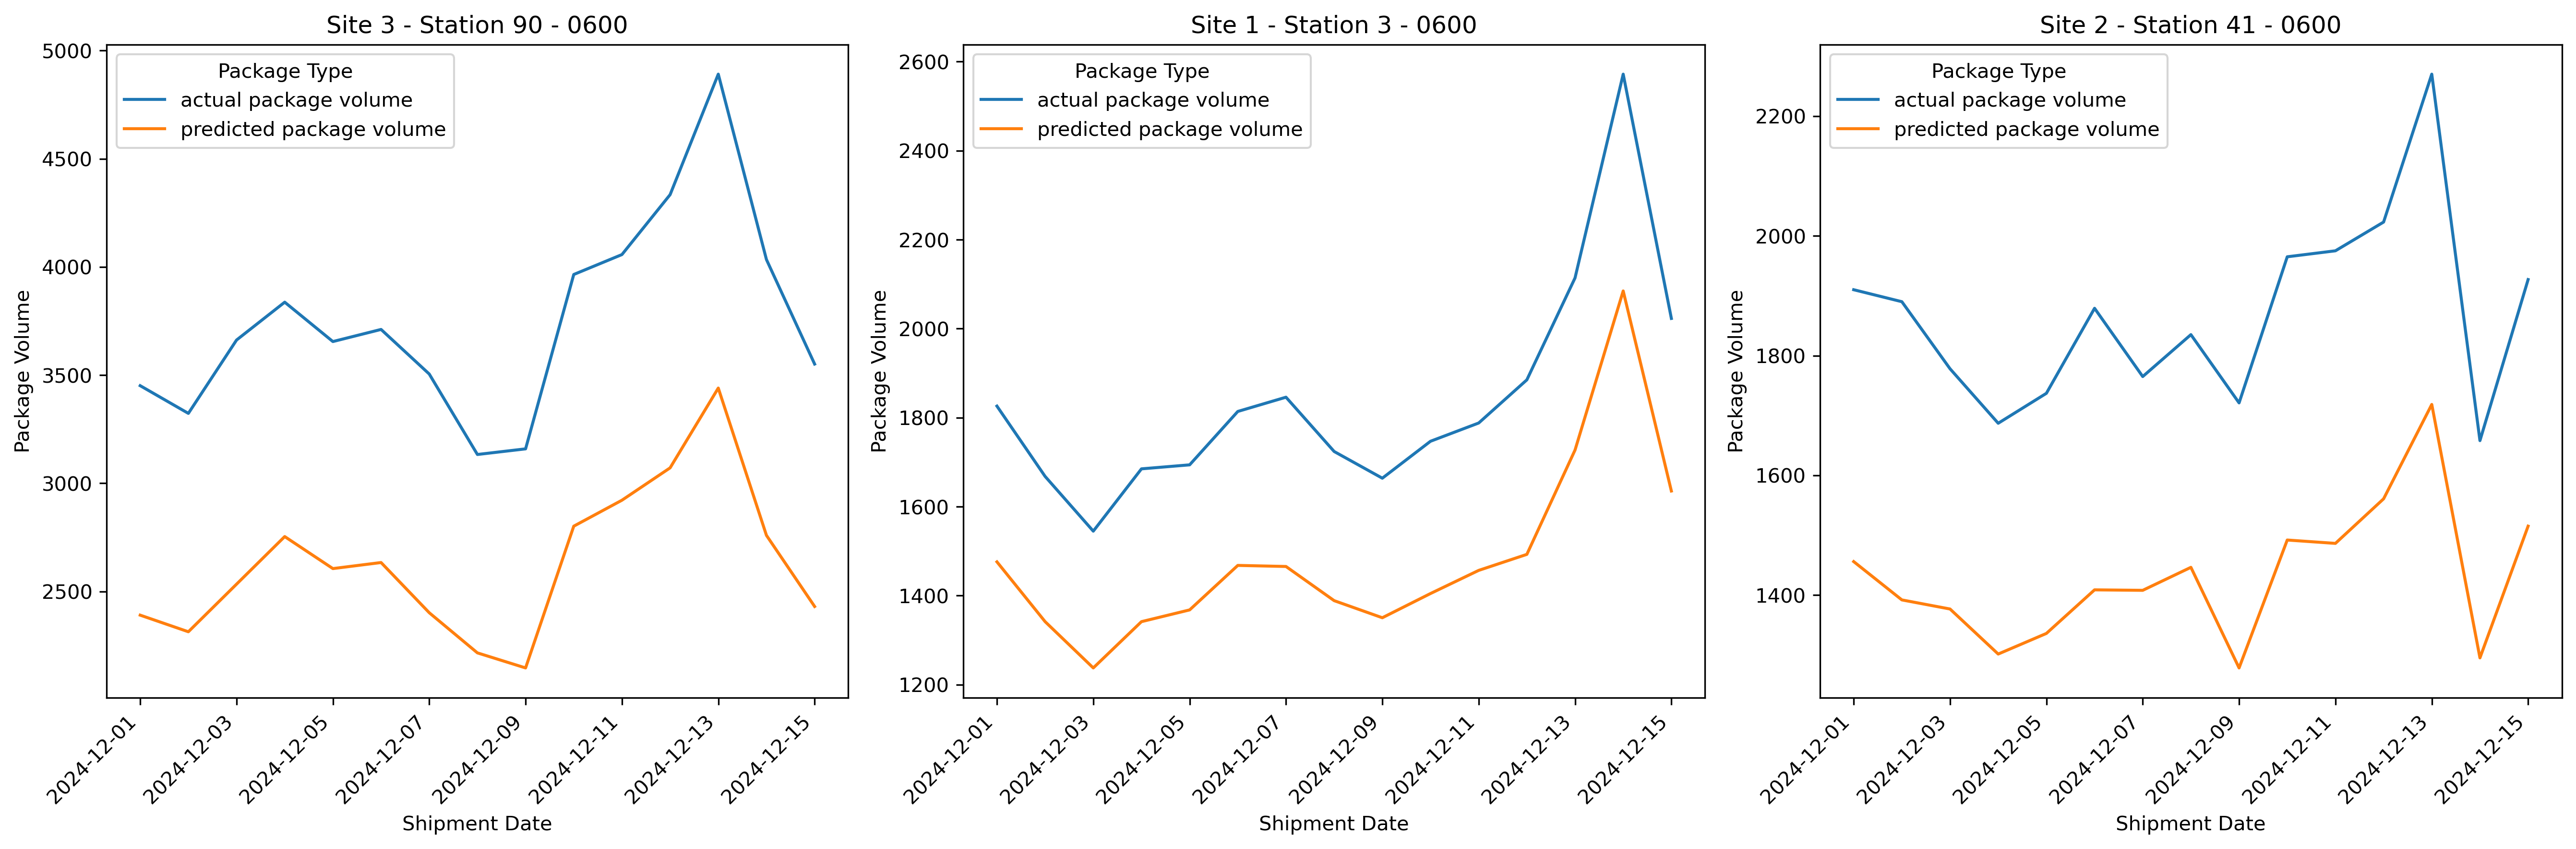
\includegraphics[width=\linewidth]{实际包裹量与预知包裹量对比.png}
	\caption{实际包裹量与预知包裹量对比}
	\label{fig:1}
\end{figure}

可以观察到,日总包裹数的实际包裹量与预知包裹量趋势完全相同,仅有绝对数量的差别。此外,二者数量之差似乎在日时间尺度上维持某个相对稳定值。为了进一步探究实际与预知包裹数量之差的稳定性,定义修正系数:
\begin{equation}
    \text{修正系数} = \frac{\text{实际包裹数}}{\text{预知包裹数}}
\end{equation}

除上述3条路线之外,另外加入路线“场地4-站点131-1400”和“场地1-站点14-1400”,5条路线在15天内修正系数的箱型图如图\ref{fig:2}所示。

\begin{figure}[htb]
	\centering
	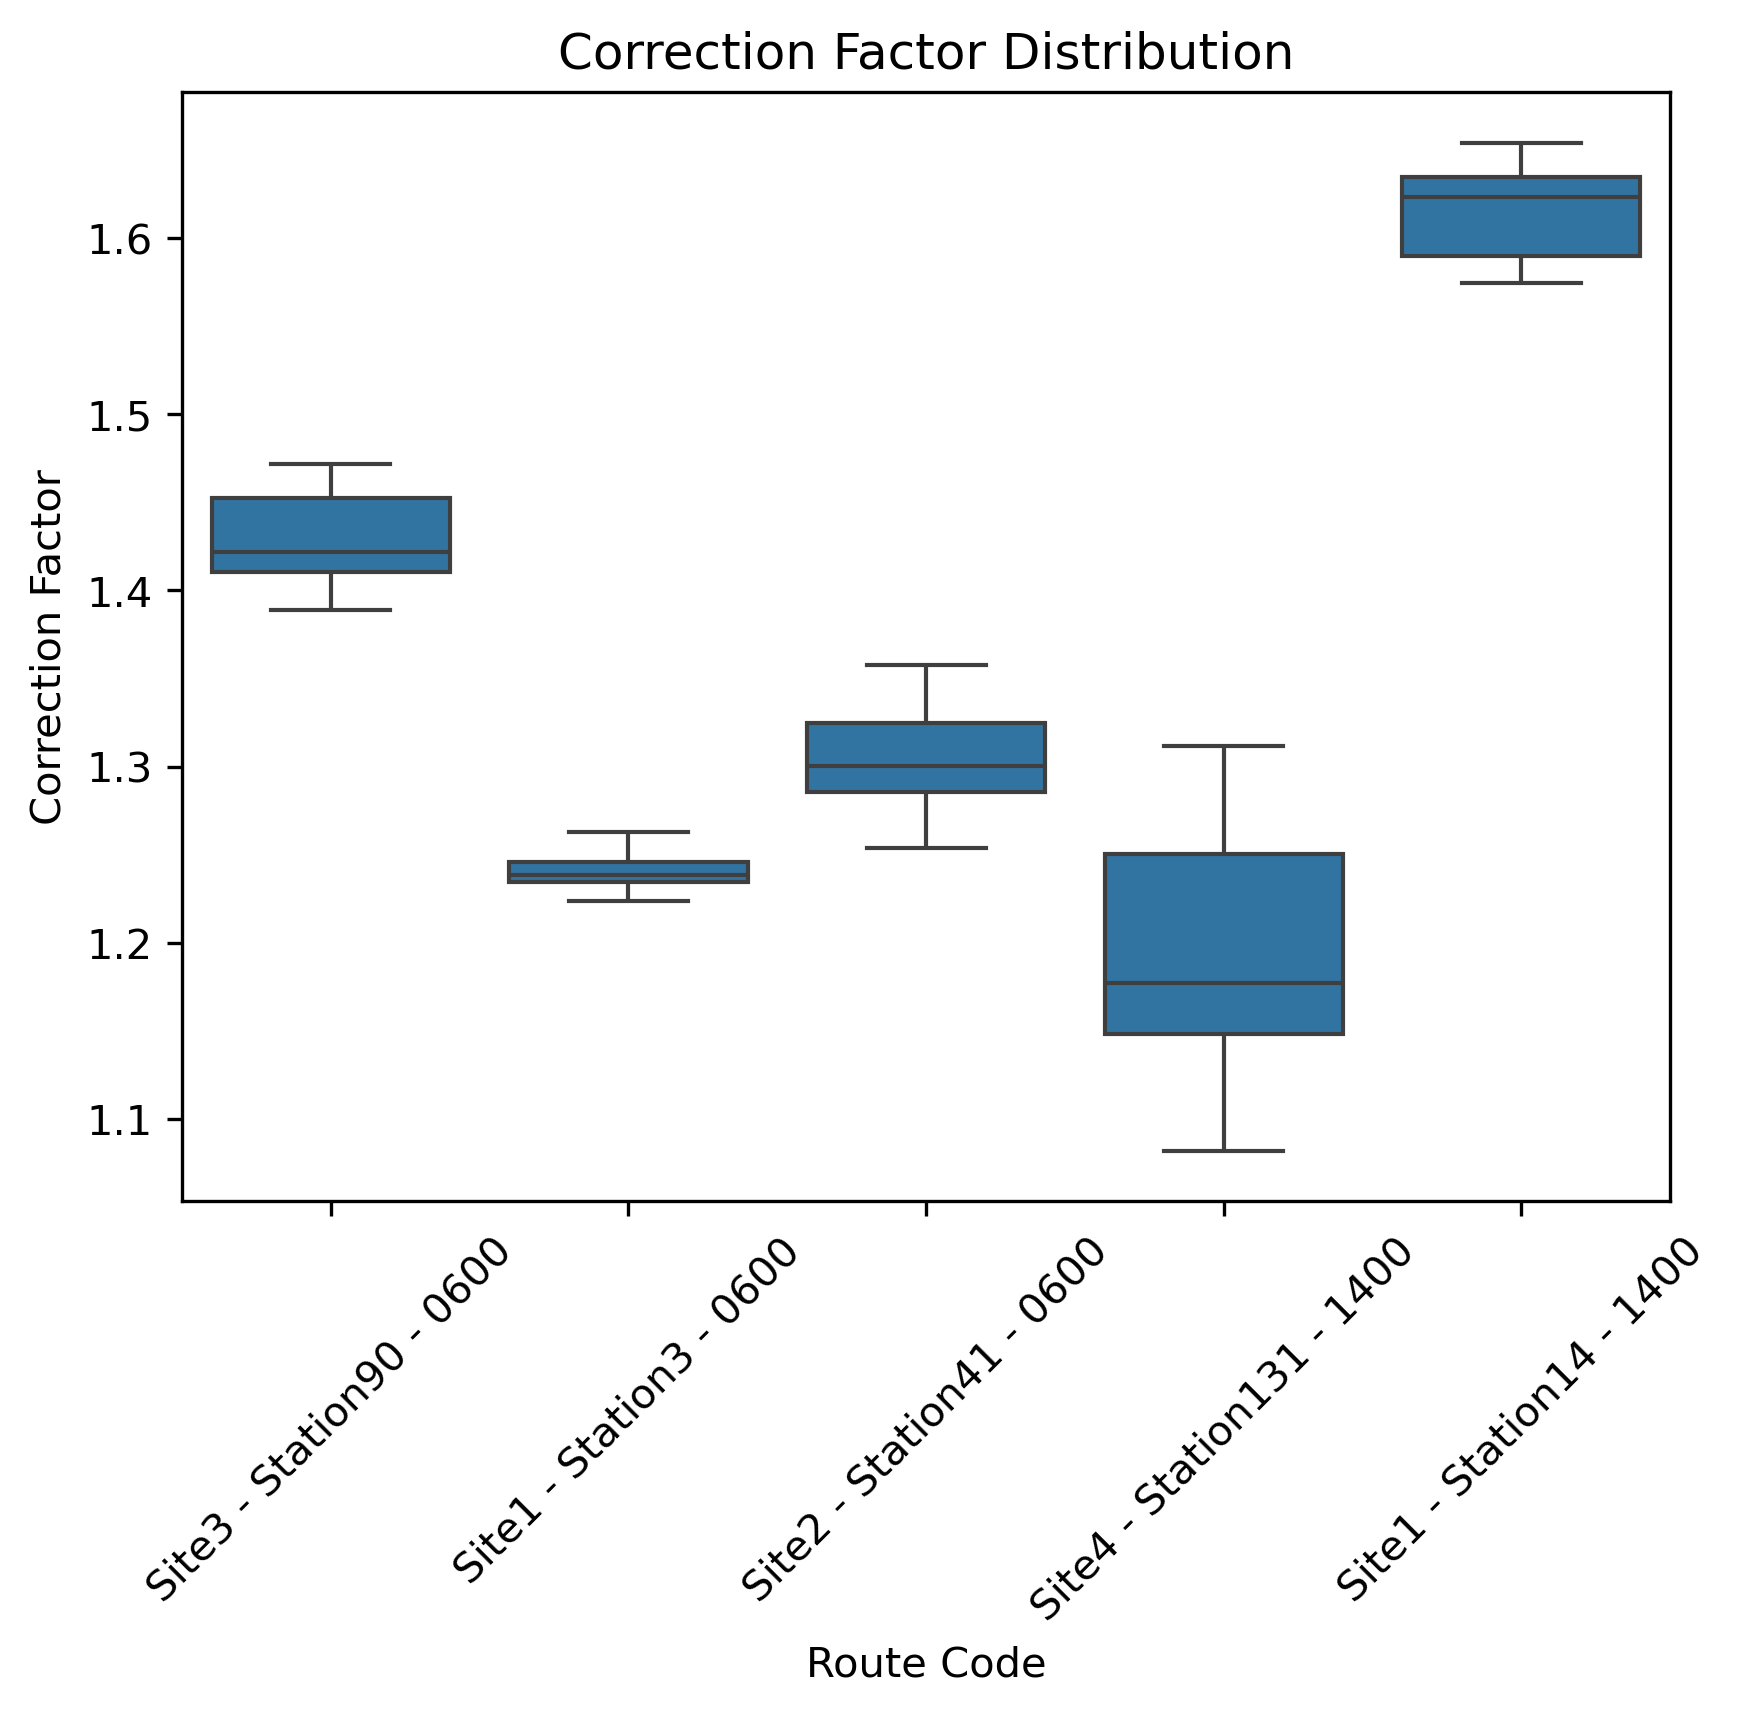
\includegraphics[width=0.8\linewidth]{修正系数分布.png}
	\caption{修正系数分布}
	\label{fig:2}
\end{figure}

对每一条路线,可以计算其修正系数的方差与标准差,为了衡量修正系数的总体变化情况,计算得到所有路线修正系数标准差的描述性统计量如表\ref{tab:1}所示:
\begin{table}[htbp]
\centering
\caption{修正系数标准差统计量描述}
\label{tab:1}
\begin{tabular}{*{7}{c}}
\toprule
统计量 & 均值 & 标准差  & 最小值 $ & 最大值  \\
\midrule
数值 & 0.1552 & 0.1664 & 0.0089 & 0.8007 \\
\bottomrule
\end{tabular}
\end{table}

由图\ref{fig:2}可知,不同路线的修正系数大小差别较大,但是同一路线不同日期的修正系数则基本稳定。由表\ref{tab:1},修正系数标准差均值为\(0.1522\),变化很小,所以图\ref{fig:2}的结论可以拓展到全体路线。

下面探究不同路线实际日总包裹数的异同。任选五条路线:“场地3-站点90-0600”、“场地3-站点68-0600”、“场地3-站点72-0600”、“场地1-站点6-0600”、“场地1-站点3-0600”,其实际包裹量折线图如图\ref{fig:3}所示。

\begin{figure}[htb]
	\centering
	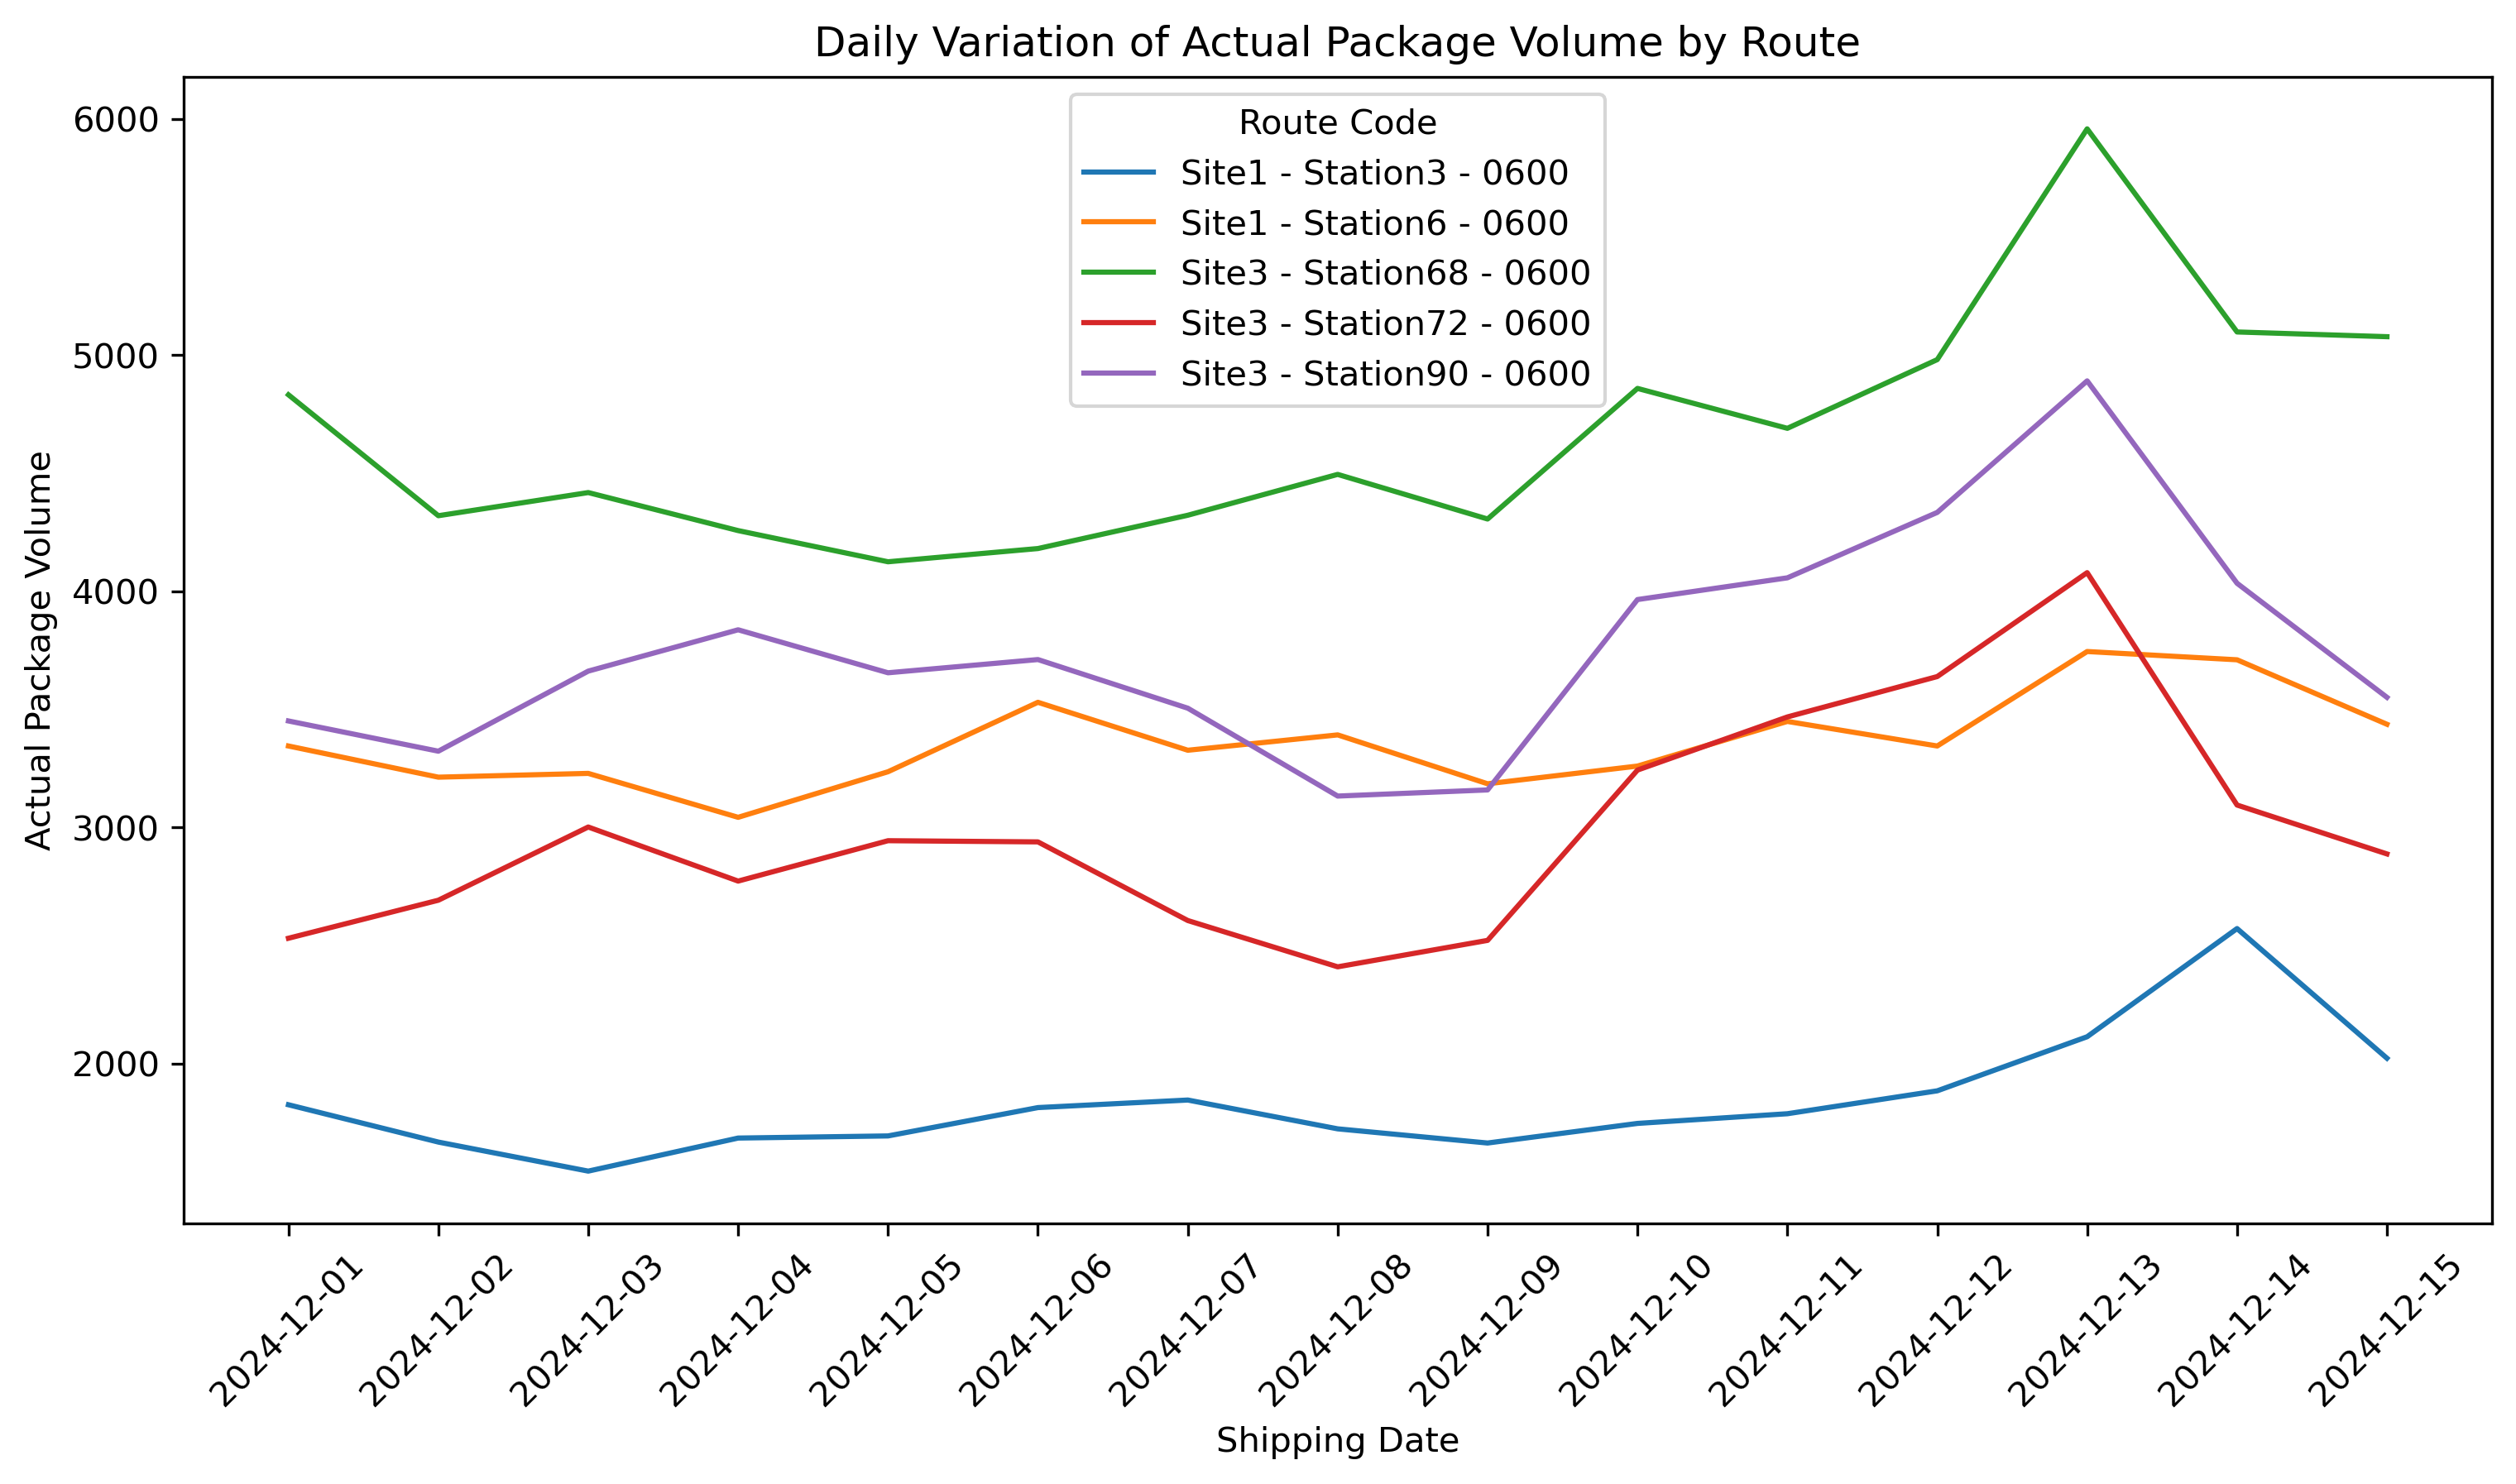
\includegraphics[width=\linewidth]{实际包裹量折线图.png}
	\caption{实际包裹量折线图}
	\label{fig:3}
\end{figure}

可以发现,不同路线总包裹量的数量和日波动均有较大差别,但是在12月10日到12月15日均遵循相同的趋势,即在12月10日到12月13日先上升,随后下降。我们猜测这与电商平台的“双十二”促销活动有关。

\subsection{各路线每10分钟包裹数}

为了有效利用附件3中12月16日的总包裹量预知值信息,我们更关注线路每10分钟包裹数与当日总包裹数的比例信息(对于发运节点为6点的路线,“当天”指从前一天21点到当前6点)。随机抽取5个路线时间点:“场地1-站点25-0600-1:00:00”、“场地4-站点126-1400-12:00:00”、“场地3-站点68-0600-22:00:00”、“场地3-站点72-0600-0:00:00”、“场地3-站点90-0600-2:00:00”,绘制其包裹占总包裹数比例的折线图如图\ref{fig:4}所示。

\begin{figure}[htb]
	\centering
	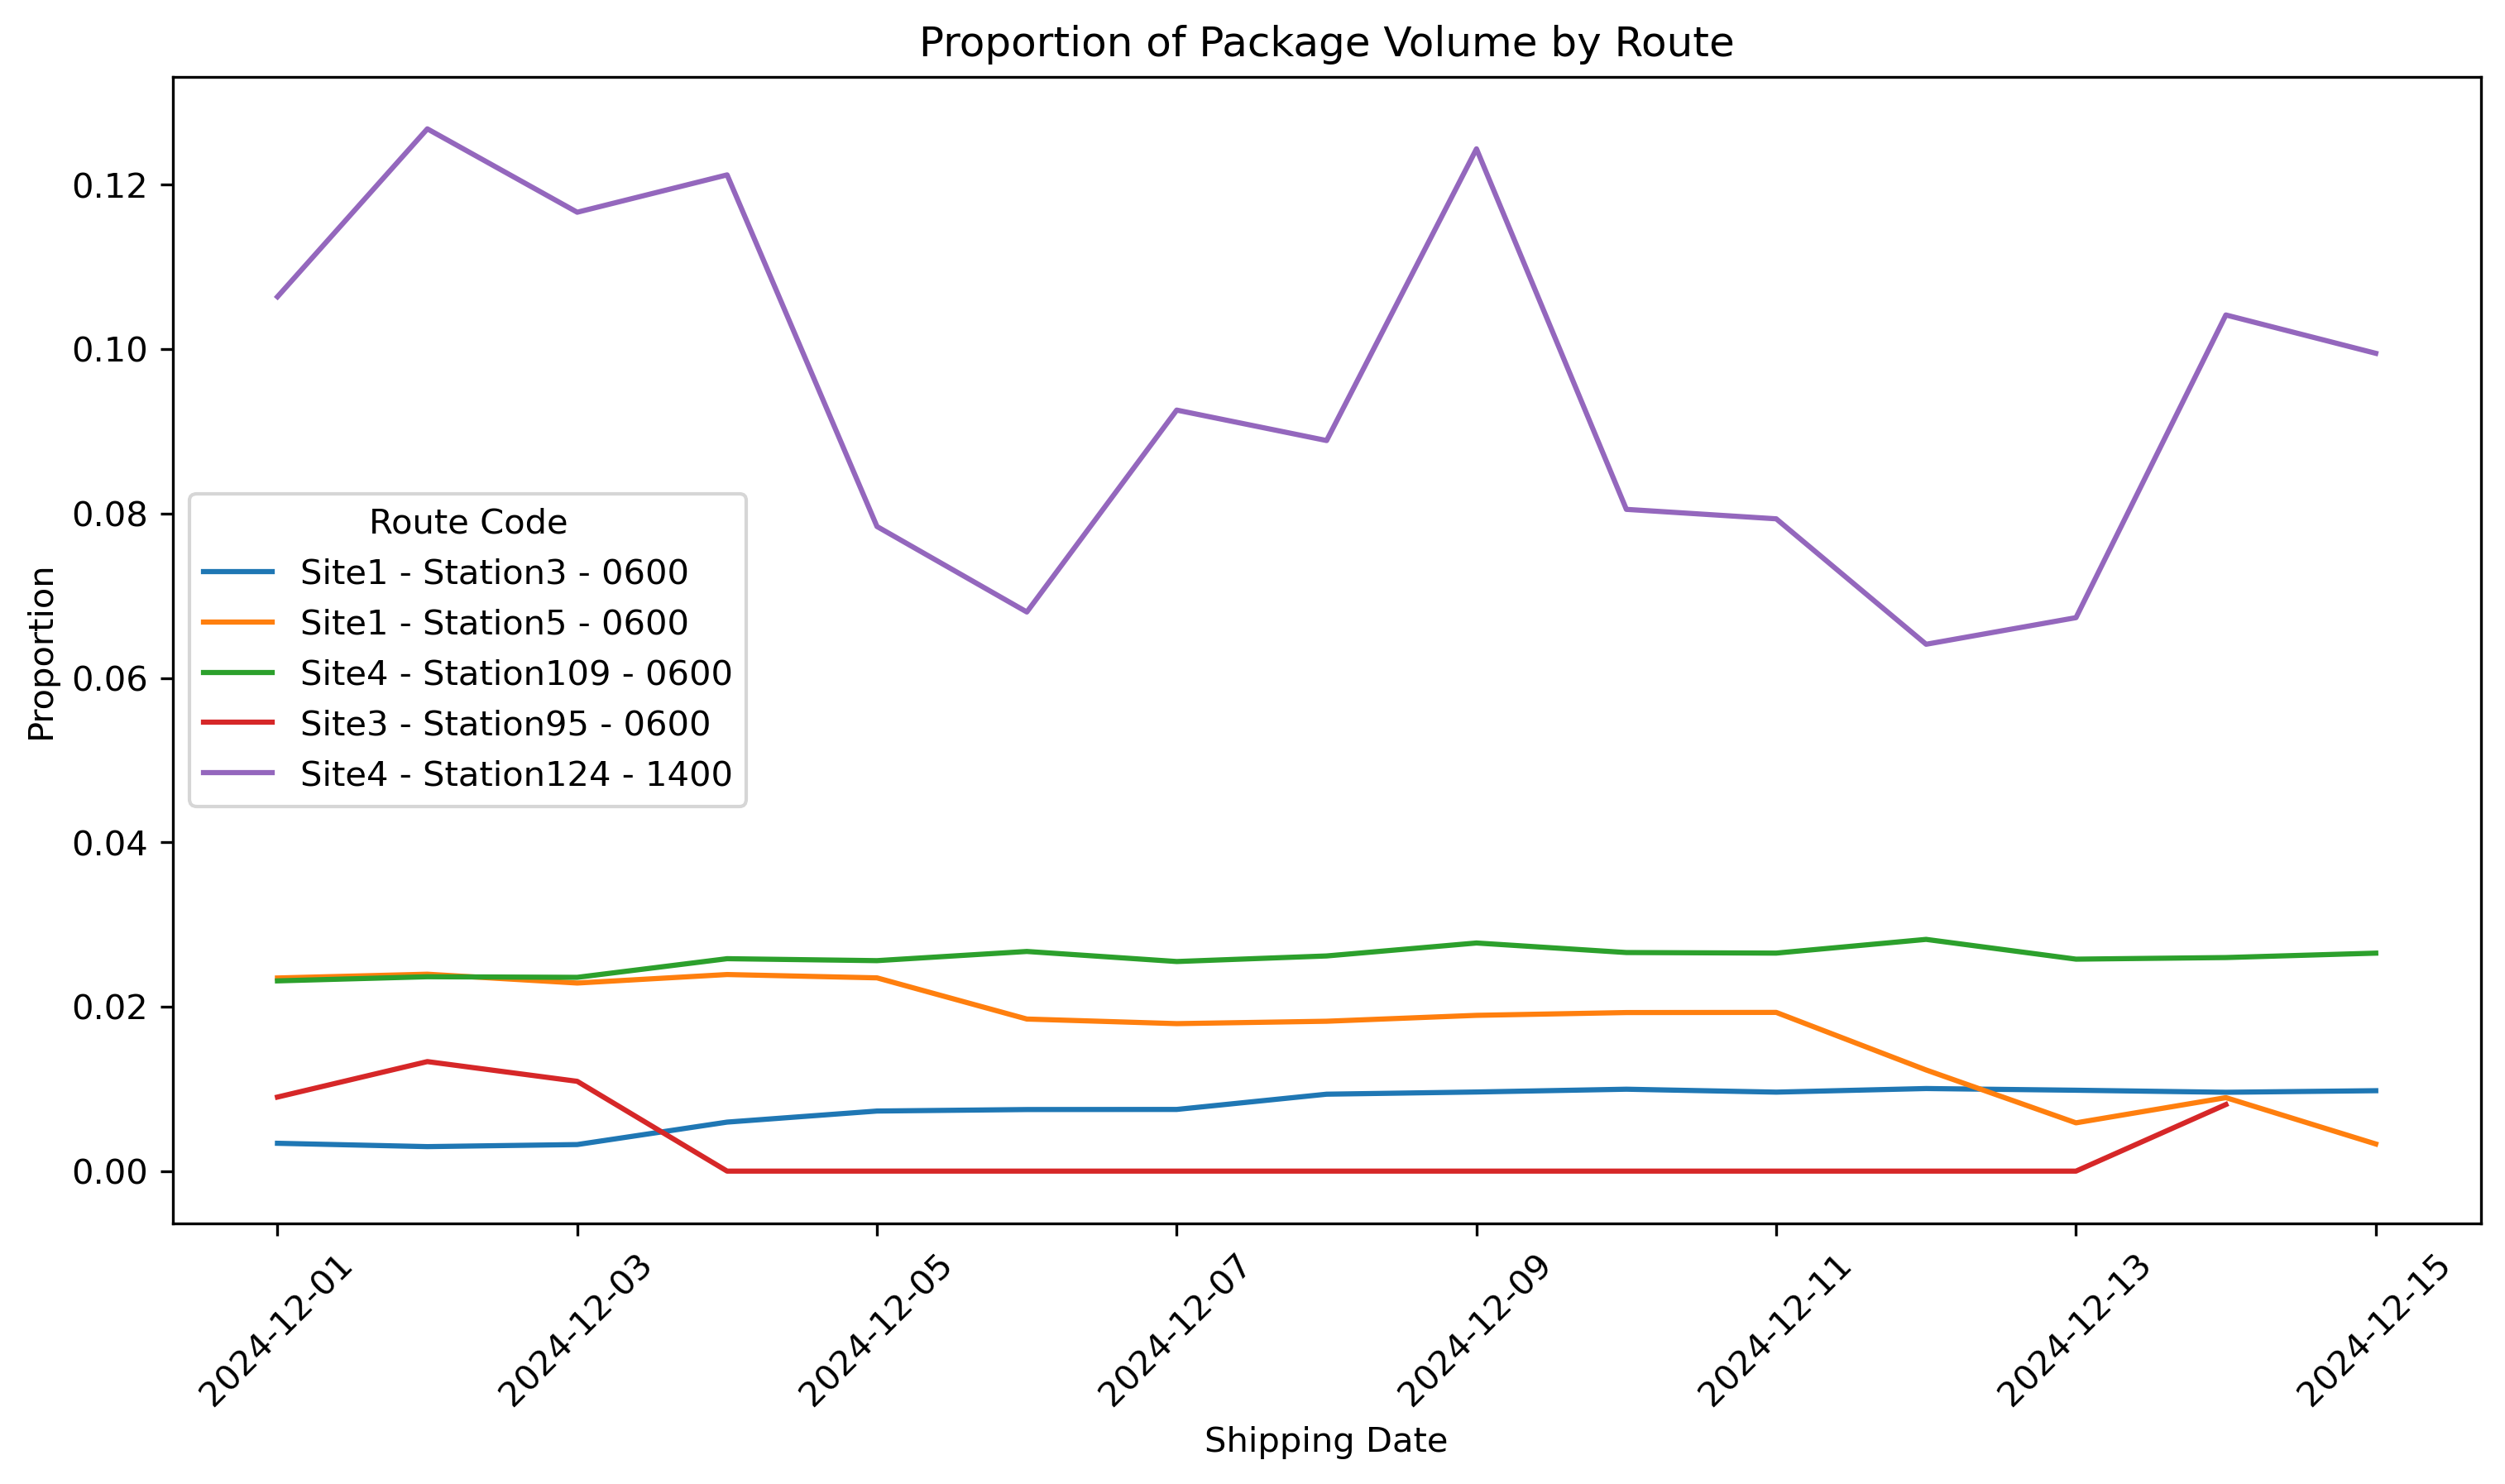
\includegraphics[width=\linewidth]{比例折线图.png}
	\caption{比例折线图}
	\label{fig:4}
\end{figure}

不同路线、不同时间的比例有明显不同,但是同一路线和时间的比例随日期的变化要么趋于稳定,要么有明显的规律性变化,这启发我们使用时间序列预测特点路线在特点时间的比例。

下面探究固定路线在一天中不同时段包裹数变化。选取路线“场地3 - 站点95 - 0600”, “场地4 - 站点109 - 0600”, “场地1 - 站点3 - 0600”, “场地3 - 站点95 - 1200”, “场地4 - 站点109 - 1200”, “场地1 - 站点3 - 1200”,日期12月1日,各路线当天包裹量变化如图\ref{fig:7}所示。

\begin{figure}[htb]
	\centering
	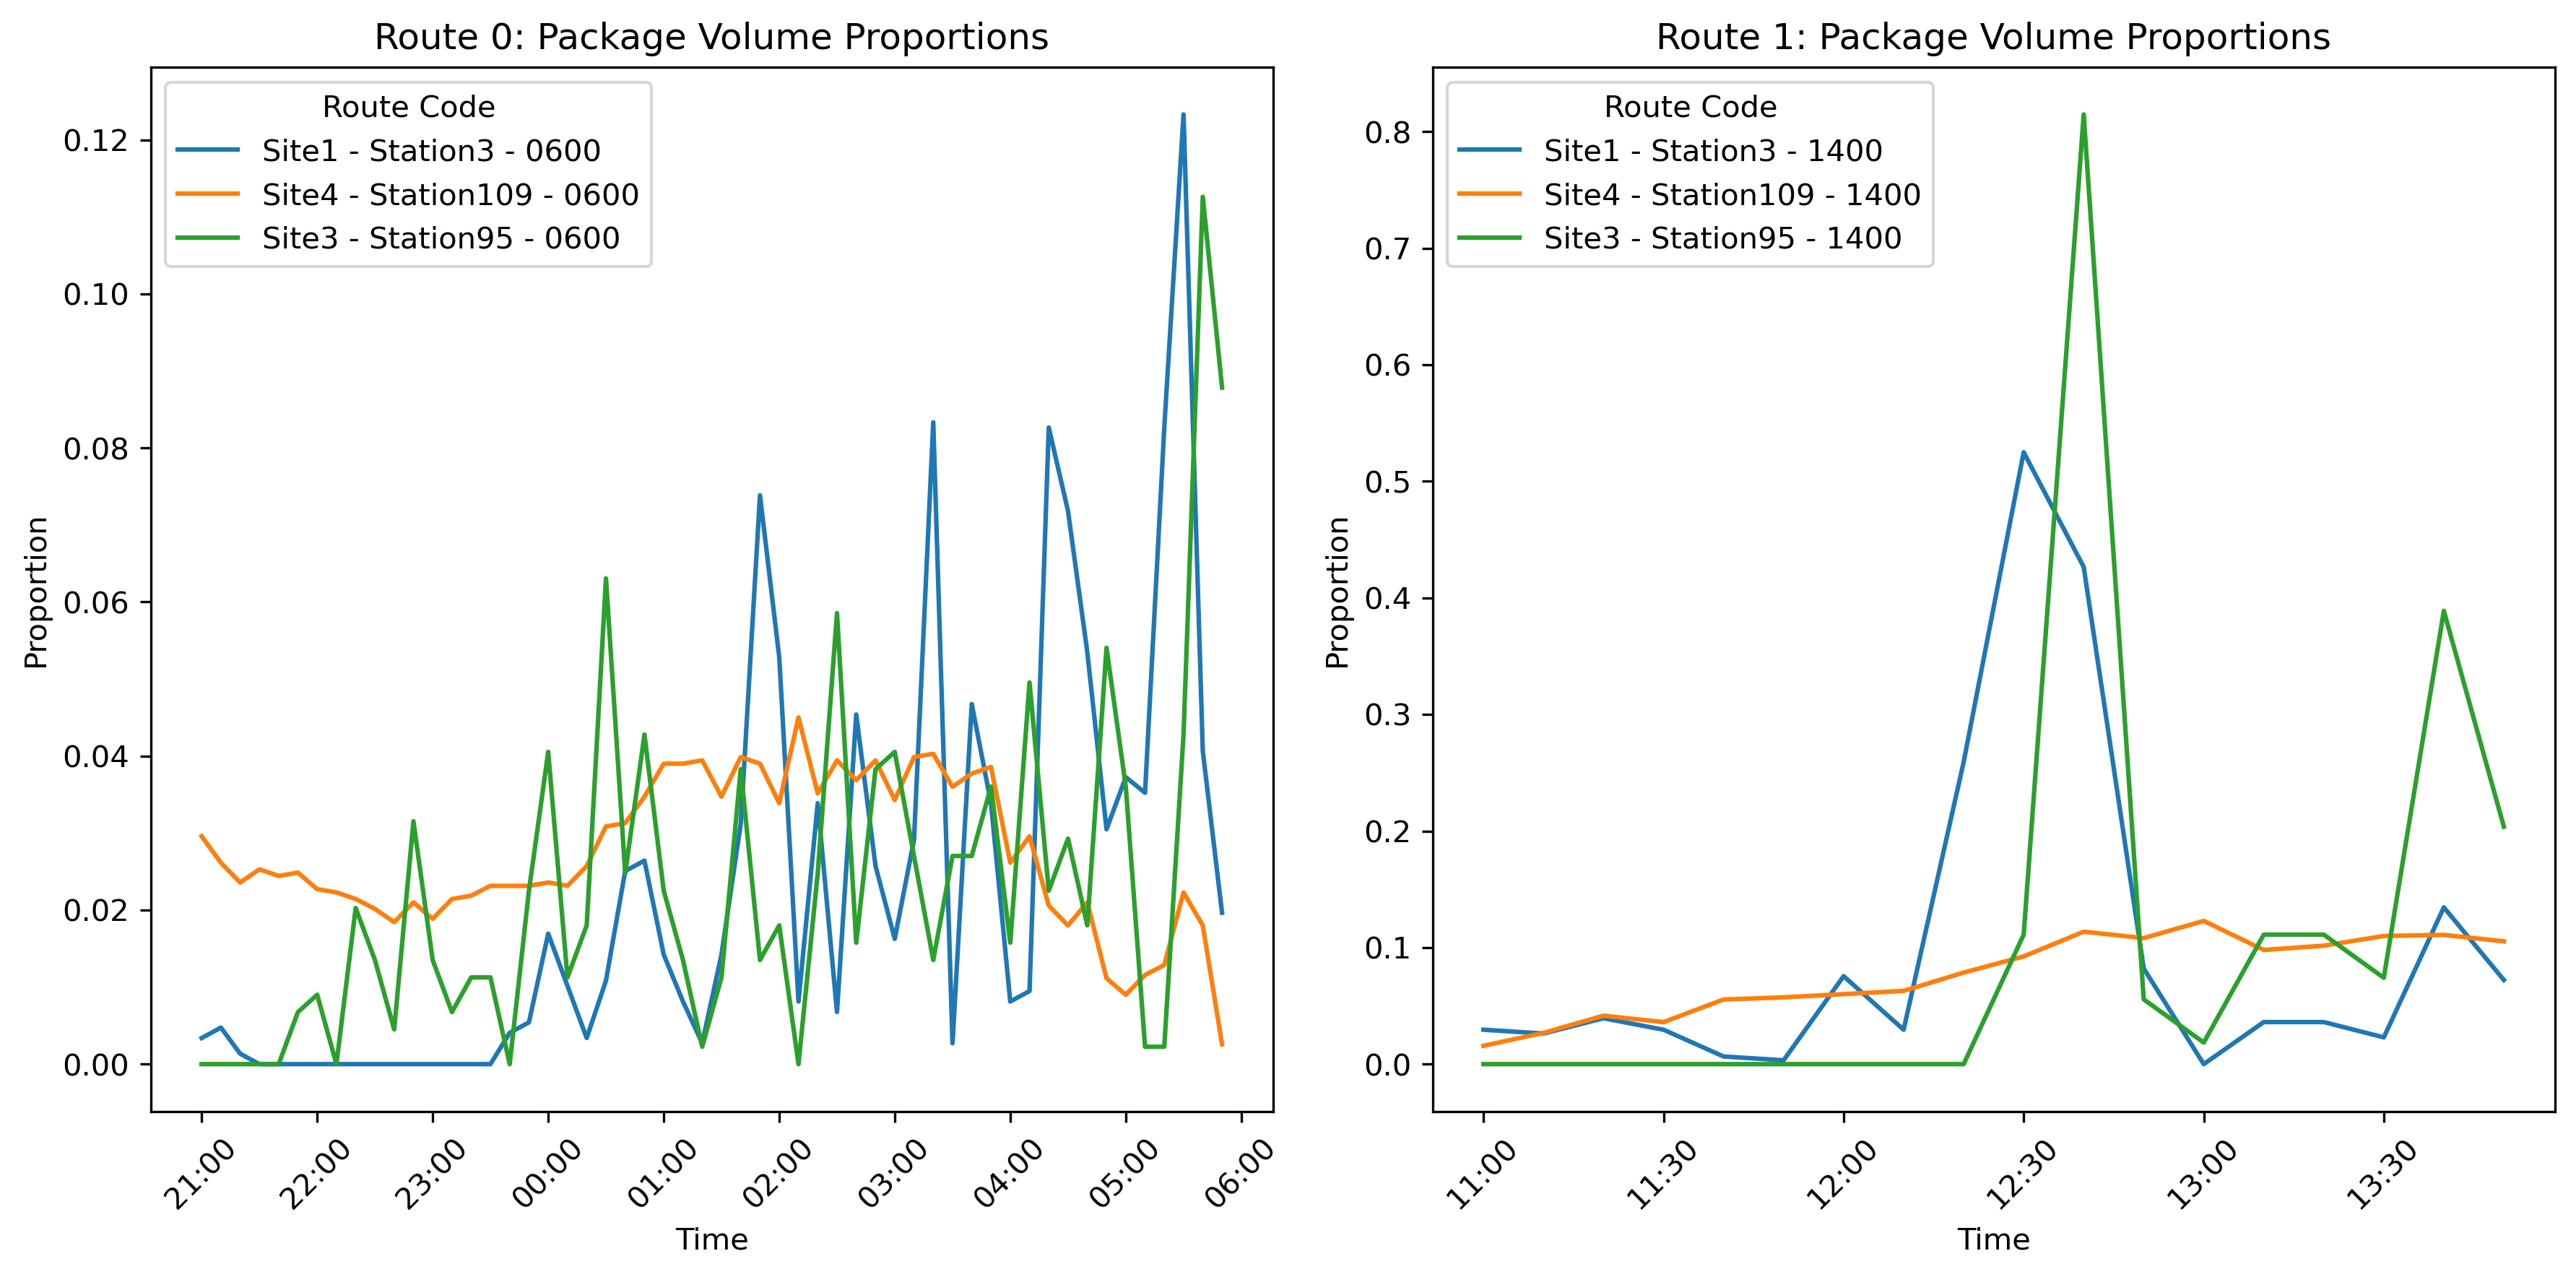
\includegraphics[width=\linewidth]{比例折线图_时间.png}
	\caption{一天中不同路线包裹量变化}
	\label{fig:7}
\end{figure}

可以观察到,同一路线一天之中包裹量变化很大,所以很难通过相邻时间段信息推断当前时间段;对于不同路线,有些会表现出相同的趋势,但也有不相关的路线。所以很难通过其他路线的包裹数或其他时间段的包裹数预测给定路线在特定时间段的包裹数。

\section{问题一模型的建立与求解}

为了有效利用附件3给出的12月16日的预知总包裹数,我们建立了从总体到10分钟粒度的两阶段预测模型。在第一阶段,使用网格搜索优化的 XGBoost 模型预测12月16日总包裹数;在第二阶段,使用Prophet时间序列预测模型以10分钟为粒度预测12月16日各时间段包裹数占总体的比例。标准化后的比例与预测的总包裹数相乘,得到各时间段包裹数。

\subsection{总包裹数的预测}
通过先前对各路线总包裹数的分析,我们知道不同路线总包裹数随日期的变化不尽相同,但是都遵循相同的趋势,所以不同路线之间的包裹数不是独立的,在预测时要尽可能利用到不同路线之间的信息关联。在后续的训练中将所有路线的数据加入模型共同训练,训练的粒度为:路线-日期。

\subsubsection{特征工程}
先前对实际总包裹量、预知总包裹量和修正系数的分析说明:预知包裹数和实际包裹数具有强相关性,所以预知包裹数是预测的最重要特征。将日期、路线主键、发运节点转化为数值型特征(12月1日对应1,以此类推),同时提取出日期中的星期特征。
根据数据的时序特性,添加滞后特征,即前一天对应线路的预知货量、实际货量和偏差。训练及预测使用的特征如表\ref{tab:2}所示。

\begin{table}[htbp]
\centering
\caption{机器学习特征列表}
\label{tab:2}
\begin{tabular}{lllp{6cm}}
\toprule
\textbf{特征名称} & \textbf{数据类型} & \textbf{取值范围} & \textbf{描述} \\
\midrule
线路主键编码 & 类别型 & [1..140] & 将每一条线路编码为数值,如“场地1-站点1”编码为1 \\
发运节点编码 & 类别型 & \{1,2\} & 将发运节点6点编码为1,14点编码为2 \\
预知货量 & 数值型 & [1, \(\infty\)) & 当天给定节点的预知货量 \\
日期 & 类别型 & [1..16] & 将16天映射到16个数字 \\
星期几 & 类别型 & [1..7] & 当天是星期几 \\
预知货量lag1 & 数值型 & [1, \(\infty\)) & 该线路前一天的预知货量\\
实际货量lag1 & 数值型 & [1, \(\infty\)) & 该路线前一天的实际货量\\
偏差 & 数值型 & [1, \(\infty\)) & 预知货量lag1 - 实际货量lag1 \\
\bottomrule
\end{tabular}
\end{table}

\subsubsection{基于网格搜索的XGBoost超参数优化方法}
提升(Boosting)算法是一类将弱学习器提升为强学习器的算法,这类算法的工作机制类似:先从初始训练集中训练出一个基学习器,再根据基学习器的表现对训练样本分布进行调整,使得先前基学习器做错的训练样本在后续受到更多关注,然后基于调整后的样本分布来训练下一个基学习器。Boost算法在算法开始时,为每一个样本赋一个相等的权重。 在每一次训练后,增加错分点的权重。

梯度提升(gradient boosting)属于Boost算法的一种,它的每一次计算都是为了减少上一次的残差(residual),而为了减少这些残差,可以在残差减少的梯度方向上建立一个新模型。所以在Gradient Boost中,每个新模型的建立是为了使得先前模型残差往梯度方向减少。

XGBoost(Extreme Gradient Boosting)是一种基于梯度提升框架的高效集成学习算法,XGBoost 通过二阶泰勒展开优化损失函数,并引入正则化项控制模型复杂度,在分类、回归及排序任务中表现卓越。然而,XGBoost的性能高度依赖于超参数组合(如学习率、树深度、正则化系数等),不当的参数选择易导致过拟合或欠拟合。

网格搜索(Grid Search)是一种穷举式超参数优化方法,其数学本质可表述为:
\begin{equation}
    \theta^* = \arg \min_{\theta \in \Theta} \mathcal{L}(f_{\theta}, D_{\text{val}})
\end{equation}
其中,\(\Theta\) 为超参数空间,\(\mathcal{L}\) 为损失函数,\(f_{\theta}\) 为参数化的XGBoost模型,\(D_{\text{val}}\) 为验证集数据。算法通过交叉验证(Cross-Validation, CV)评估每个参数组合 \(\theta_i\) 的泛化性能,最终选择验证误差最小的配置 \(\theta^*\)。基于网格搜索方法的 XGBoost 模型可以系统性地遍历预设参数空间,以确定全局最优超参数配置。

\begin{figure}[htb]
	\centering
	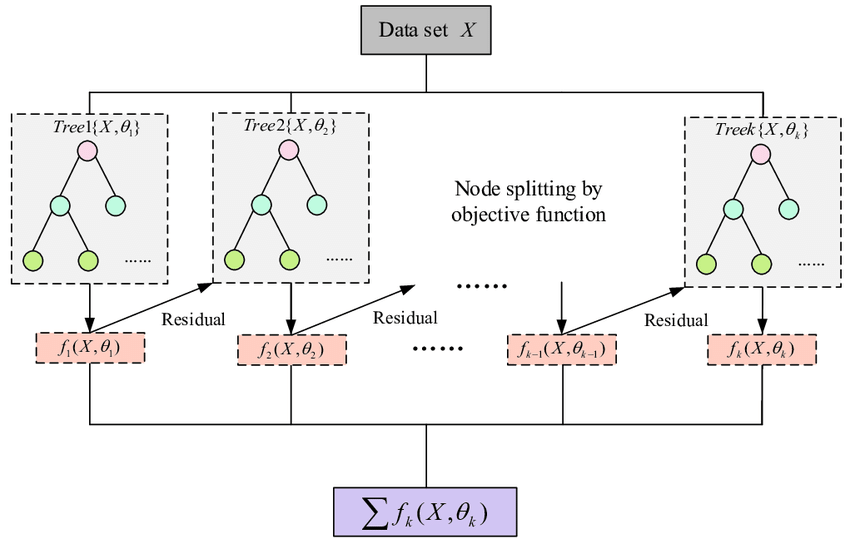
\includegraphics[width=0.8\linewidth]{XGBoost.png}
	\caption{XGBoost原理图}
	\label{fig:6}
\end{figure}

\begin{figure}[htb]
	\centering
	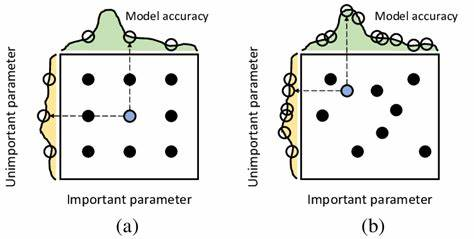
\includegraphics[width=0.8\linewidth]{GridSearch.jpg}
	\caption{网格搜索原理图}
	\label{fig:5}
\end{figure}

\subsubsection{模型训练与评估}
   在训练之前,选取对模型性能敏感的6类XGBoost核心参数构建网格空间:
    \begin{equation}
    \Theta = \left\{ 
       \begin{aligned}
       & \eta \in [0.01, 0.1], \ 
       \gamma \in [0, 0.5], \ 
       \lambda \in [1, 10], \\
       & \text{max\_depth} \in \{3, 5, 7\}, \ 
       \text{subsample} \in [0.6, 1.0], \\
       & \text{colsample\_bytree} \in [0.6, 1.0]
       \end{aligned} 
    \right\}
    \end{equation}
   其中,\(\eta\) 为学习率,\(\gamma\) 为分裂最小损失下降阈值,\(\lambda\) 为L2正则化系数。

考虑到数据的时序性特征,要注意时间依赖性,即未来数据不能影响过去数据的建模,所以在划分训练集和测试集时,将12月1日到12月14日的数据作为训练集,12月15日的数据作为测试集,并最终预测12月16日数据。

使用网格搜索获取的最优参数如表\ref{tab:5}所示。

\begin{table}[h]
\centering
\caption{XGBoost 最优参数}
\label{tab:5}
\begin{tabular}{|c|c|c|c|c|c|c|}
\hline
\textbf{Parameter} & colsample bytree & learning rate & max depth & n estimators & reg & subsample \\ \hline
\textbf{Value} & 1.0 & 0.1 & 5 & 150 & 10 & 0.8 \\ \hline
\end{tabular}
\end{table}

使用模型内置的"feature\_importances\_"参数,得到的特征重要性如图\ref{fig:8}所示。

\begin{figure}[htb]
	\centering
	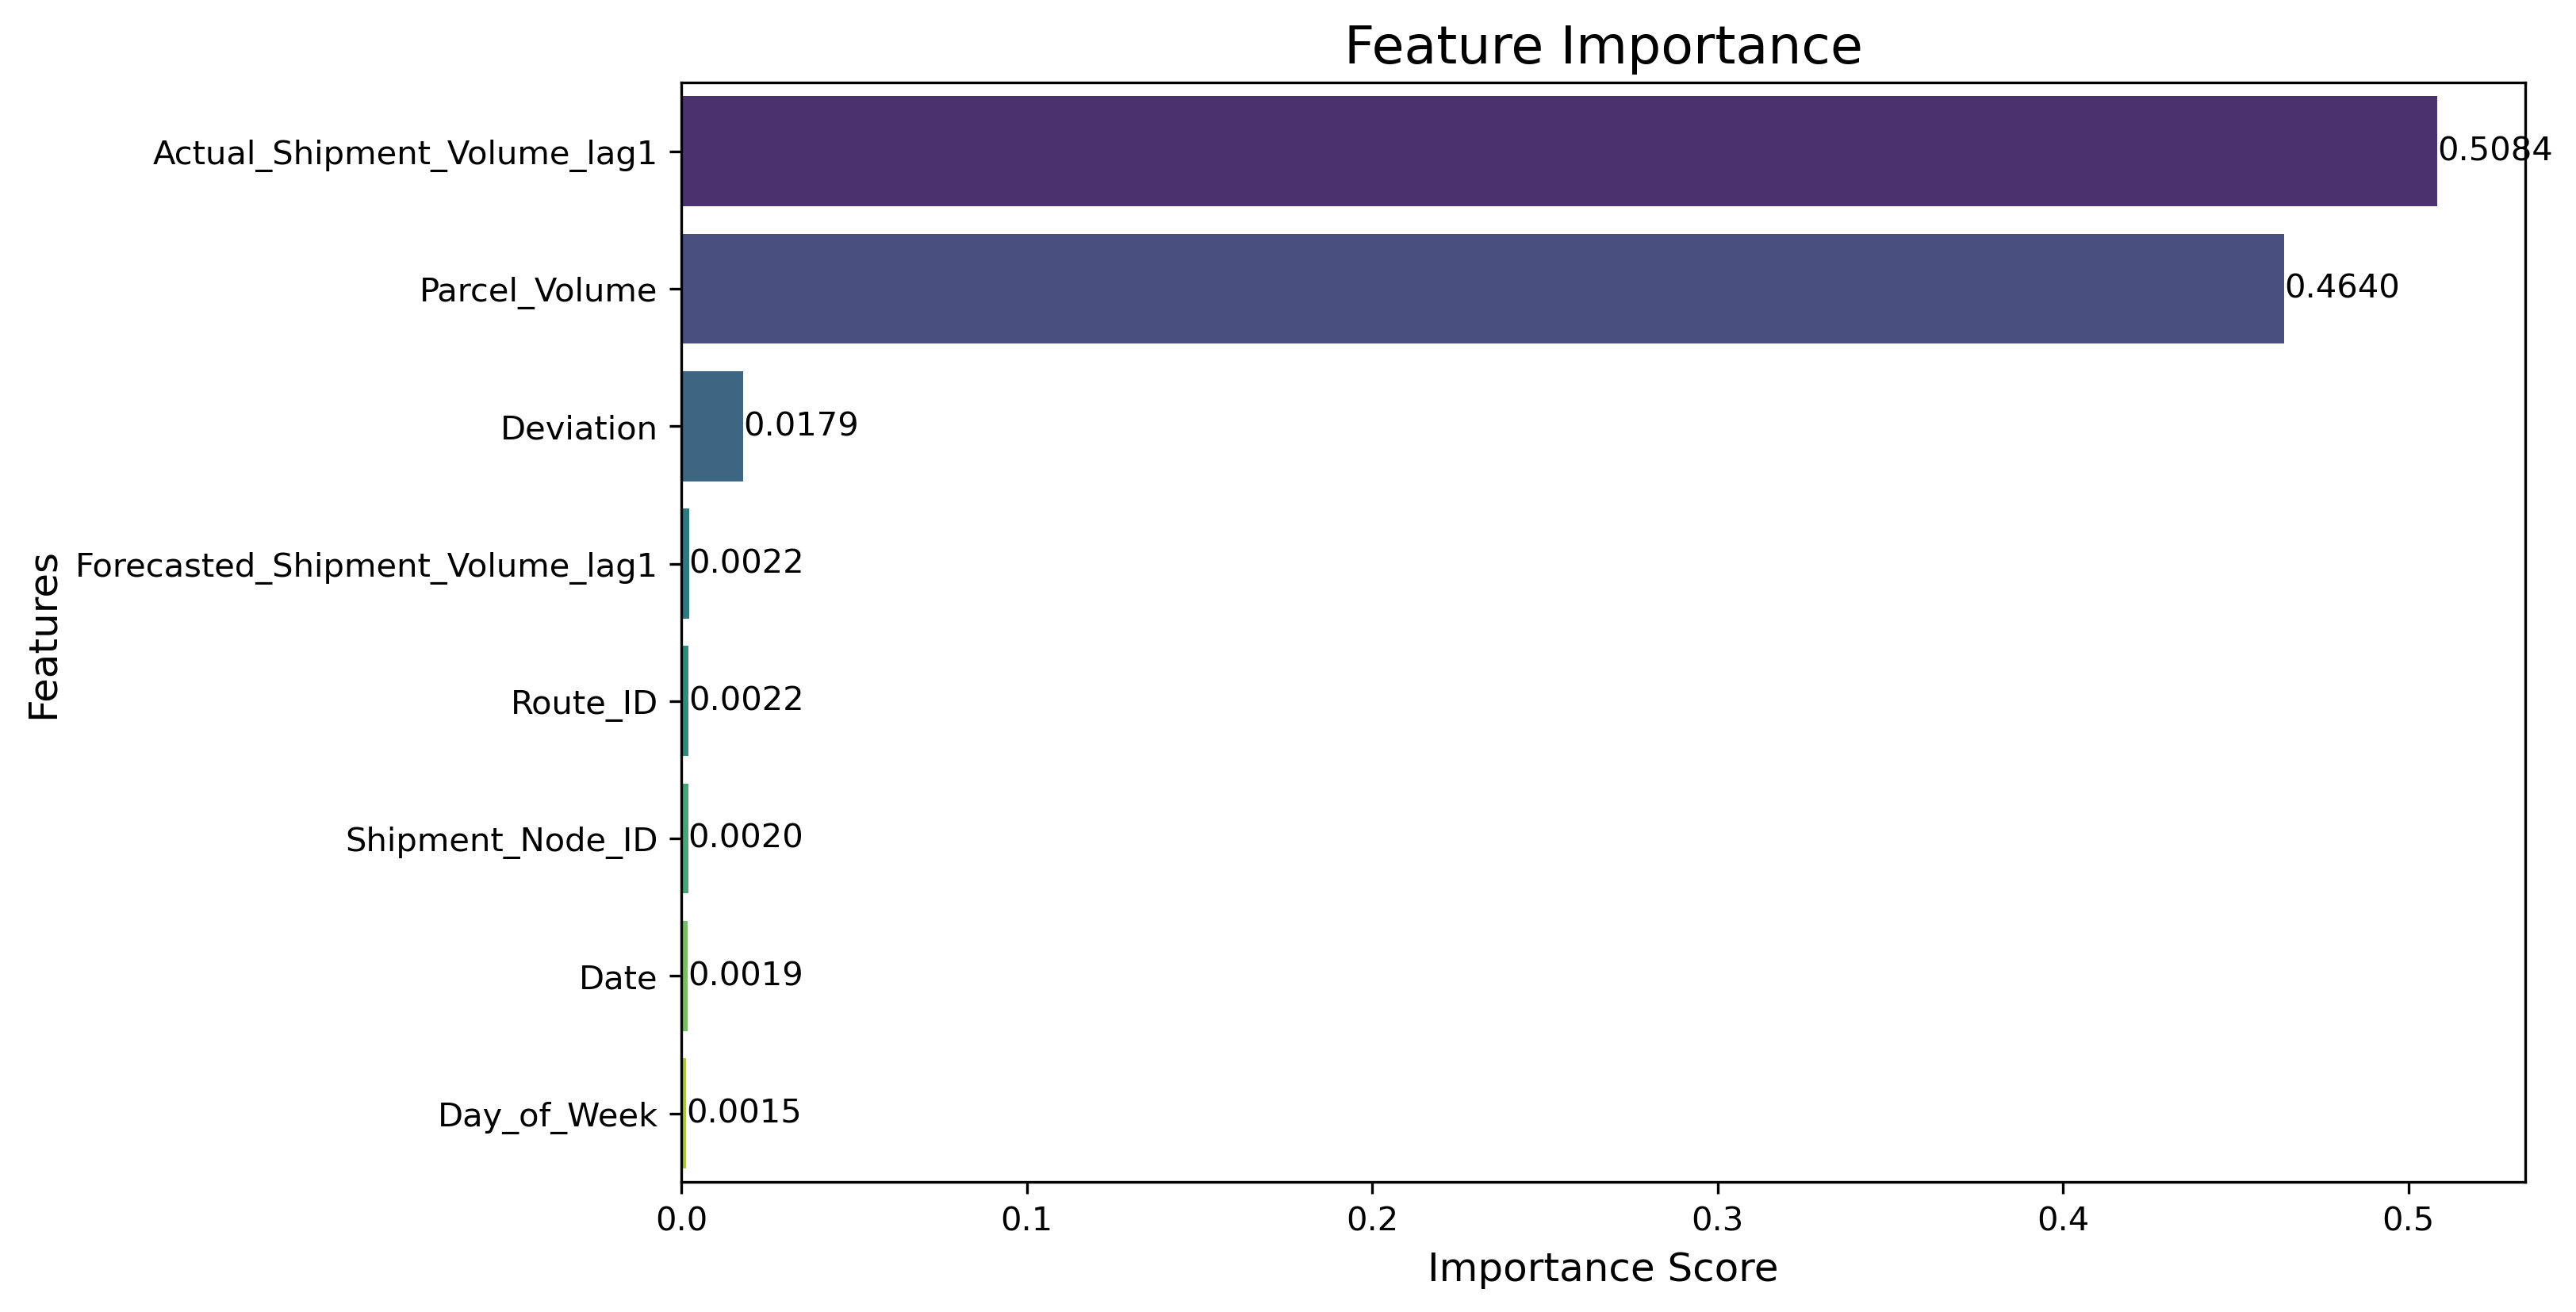
\includegraphics[width=\linewidth]{特征重要性.png}
	\caption{特征重要性}
	\label{fig:8}
\end{figure}

可见延迟一天的实际货量与当天的预知货量是预测最重要的根据,这与“数据侧写”一章中对预知货量的分析相同,而前一天的实际货量也显然对当天有很大影响。这体现了模型预测的合理性。

模型在测试集评估的结果如表\ref{tab:3}所示。

\begin{table}[h]
\centering
\caption{模型评估结果}
\label{tab:3}
\begin{tabular}{|c|c|c|c|c|}
\hline
\textbf{指标} & MAE & MSE & RMSE & R\textsuperscript{2} \\ \hline
\textbf{值}   & 90.7044 & 20181.1675 & 142.0604 & 0.9906 \\ \hline
\end{tabular}
\end{table}

\(R^2 = 0.9906\),说明数据的拟合效果极佳,模型有效地捕捉到了数据的结构,同时\(\text{MAE} = 90.7044\),各路线平均总包裹数\(\bar{n} = 1821\),所以平均相对误差\(\text{MRE} = \frac{\bar{n}}{\text{MAE}} = 4.98\%\)。考虑到不同路线的差异以及路线时序变化波动较大,该模型的预测效果优异。

使用模型预测12月16日总包裹数,部分线路的预测值如表\ref{tab:4}所示,完整结果见结果表1。
\begin{table}[h]
\centering
\caption{线路编码与预测总货量}
\label{tab:4}
\begin{tabular}{|c|c|}
\hline
\textbf{线路编码} & \textbf{预测总货量} \\ \hline
场地1 - 站点1 - 0600 & 3240 \\ \hline
场地1 - 站点1 - 1400 & 1181 \\ \hline
场地1 - 站点10 - 0600 & 1151 \\ \hline
场地1 - 站点10 - 1400 & 366 \\ \hline
场地1 - 站点11 - 0600 & 2199 \\ \hline
场地1 - 站点11 - 1400 & 367 \\ \hline
场地1 - 站点12 - 0600 & 3196 \\ \hline
场地1 - 站点12 - 1400 & 1048 \\ \hline
\end{tabular}
\end{table}

\subsection{各区间包裹数的预测}
根据先前的分析,该阶段的目标是预测12月16日各路线在各时间段(以10分钟为粒度)的包裹数占总包裹数的比例。由于(具体分析见第二章):
\begin{enumerate}
    \item 不同路线在一天中包裹数的变化情况不一定有关联;
    \item 同一路线在一天中包裹数的波动情况可能非常大,
\end{enumerate}
所以将不同路线、不同时间段的数据共同加入模型预测,不仅无法捕捉共同特征,反而会使得数据之间相互干扰,降低预测效果。

又因为同一路线固定时间段包裹数随日期的变化要么趋于稳定,要么有明显的规律性变化(如图\ref{fig:4}),所以可以利用时间序列预测包裹数比例。

\subsubsection{Prophet 时间序列模型}

Prophet是由Facebook提出的开源时间序列预测模型,专为具有显著周期性特征及节假日效应的时间序列数据设计。该模型通过可解释的参数化结构,将时间序列分解为趋势项、季节性项和节假日效应项的组合。
  
Prophet采用加法模型框架,其数学表达式为: 

\begin{equation}
    y(t) = g(t) + s(t) + h(t) + \varepsilon_t
\end{equation}

其中,\( g(t) \) 表示趋势项,描述时间序列的长期变化规律;\( s(t) \) 为周期性季节项,捕捉日、周、年等固定周期的波动模式;\( h(t) \) 为节假日及特殊事件项,用于刻画已知日期的影响;\( \varepsilon_t \) 为误差项,服从正态分布。

具体而言,
\begin{enumerate}
    \item 使用分段线性回归捕捉具有明显拐点的趋势:
    \begin{equation}
             g(t) = \left( k + \boldsymbol{a}(t)^T \boldsymbol{\delta} \right) t + \left( m + \boldsymbol{a}(t)^T \boldsymbol{\gamma} \right)
    \end{equation}
    \item 采用傅里叶级数逼近周期性模式:
    \begin{equation}
          s(t) = \sum_{n=1}^N \left[ a_n \cos\left(\frac{2\pi n t}{T}\right) + b_n \sin\left(\frac{2\pi n t}{T}\right) \right]
    \end{equation}
    \item 通过设置日期窗函数量化突发事件影响:
    \begin{equation}
        h(t) = \sum_{i=1}^L \kappa_i \cdot \mathbb{I}_{\{ t \in D_i \}}
    \end{equation}
    其中 \( D_i \) 表示第 \( i \) 个节假日的时间窗口,\( \kappa_i \) 为对应影响系数。
\end{enumerate}
 
所以 Phrophet 模型特别适用于数据量较少且数据波动较大的场景。

\subsubsection{模型训练与评估}

对每一条路线在每一时间段的比例分别进行预测,各路线及各时间段之间相互独立。每次预测都根据12月1日到12月15日的包裹比例数据来预测12月16日的比例。

在评估模型预测效果时,使用Prophet内置的交叉验证程序,考虑到数据量不大,初始参数设定为:初始训练期长度\(initial = 7\),切割间隔\(period = 1\),预测窗口长度\(horizon = 1\),单位均为天。

由于训练的次数非常多(共有\(10080\)次训练),所以只展示性能指标的统计量,如表\ref{tab:6}所示。

\begin{table}[htbp]
\centering
\caption{Descriptive Statistics of Forecast Accuracy Metrics}
\label{tab:metrics}
\begin{tabular}{lrrrrrrrr}
\toprule
Metric & Mean & Std Dev & Min & 25\% & Median & 75\% & IQR & Max \\
\midrule
MSE    & 0.0005 & 0.0022 & 0.0000 & 0.0000 & 0.0000 & 0.0001 & 0.0001 & 0.0182 \\
RMSE   & 0.0123 & 0.0195 & 0.0002 & 0.0039 & 0.0068 & 0.0112 & 0.0072 & 0.1348 \\
MAE    & 0.0101 & 0.0161 & 0.0001 & 0.0032 & 0.0058 & 0.0090 & 0.0058 & 0.1023 \\
MAPE   & 0.1410 & 0.2158 & 0.0319 & 0.0763 & 0.1115 & 0.1756 & 0.1493 & 0.5664 \\
\bottomrule
\end{tabular}
\end{table}

模型的平均MAE和RMSE均维持在\(0.01\)的水平,中位数在\(0.06\)左右,MAPE显示模型预测相对误差的中位数约为\(10\%\)。考虑到大多数站点的波动程度较大,相邻日期之间的比例波动可以达到\(40\%\)以上,这一误差是可以接受的。

\subsubsection{预测结果}
为了展示预测效果,我们首先选取“场地 3 - 站点 83 – 0600” 在 “00:10:00” 和“场
地 3 - 站点 83 – 1400” 在 “12:00:00” 时段的预测效果,如图\ref{fig:9}所示。

\begin{figure}[htb]
	\centering
	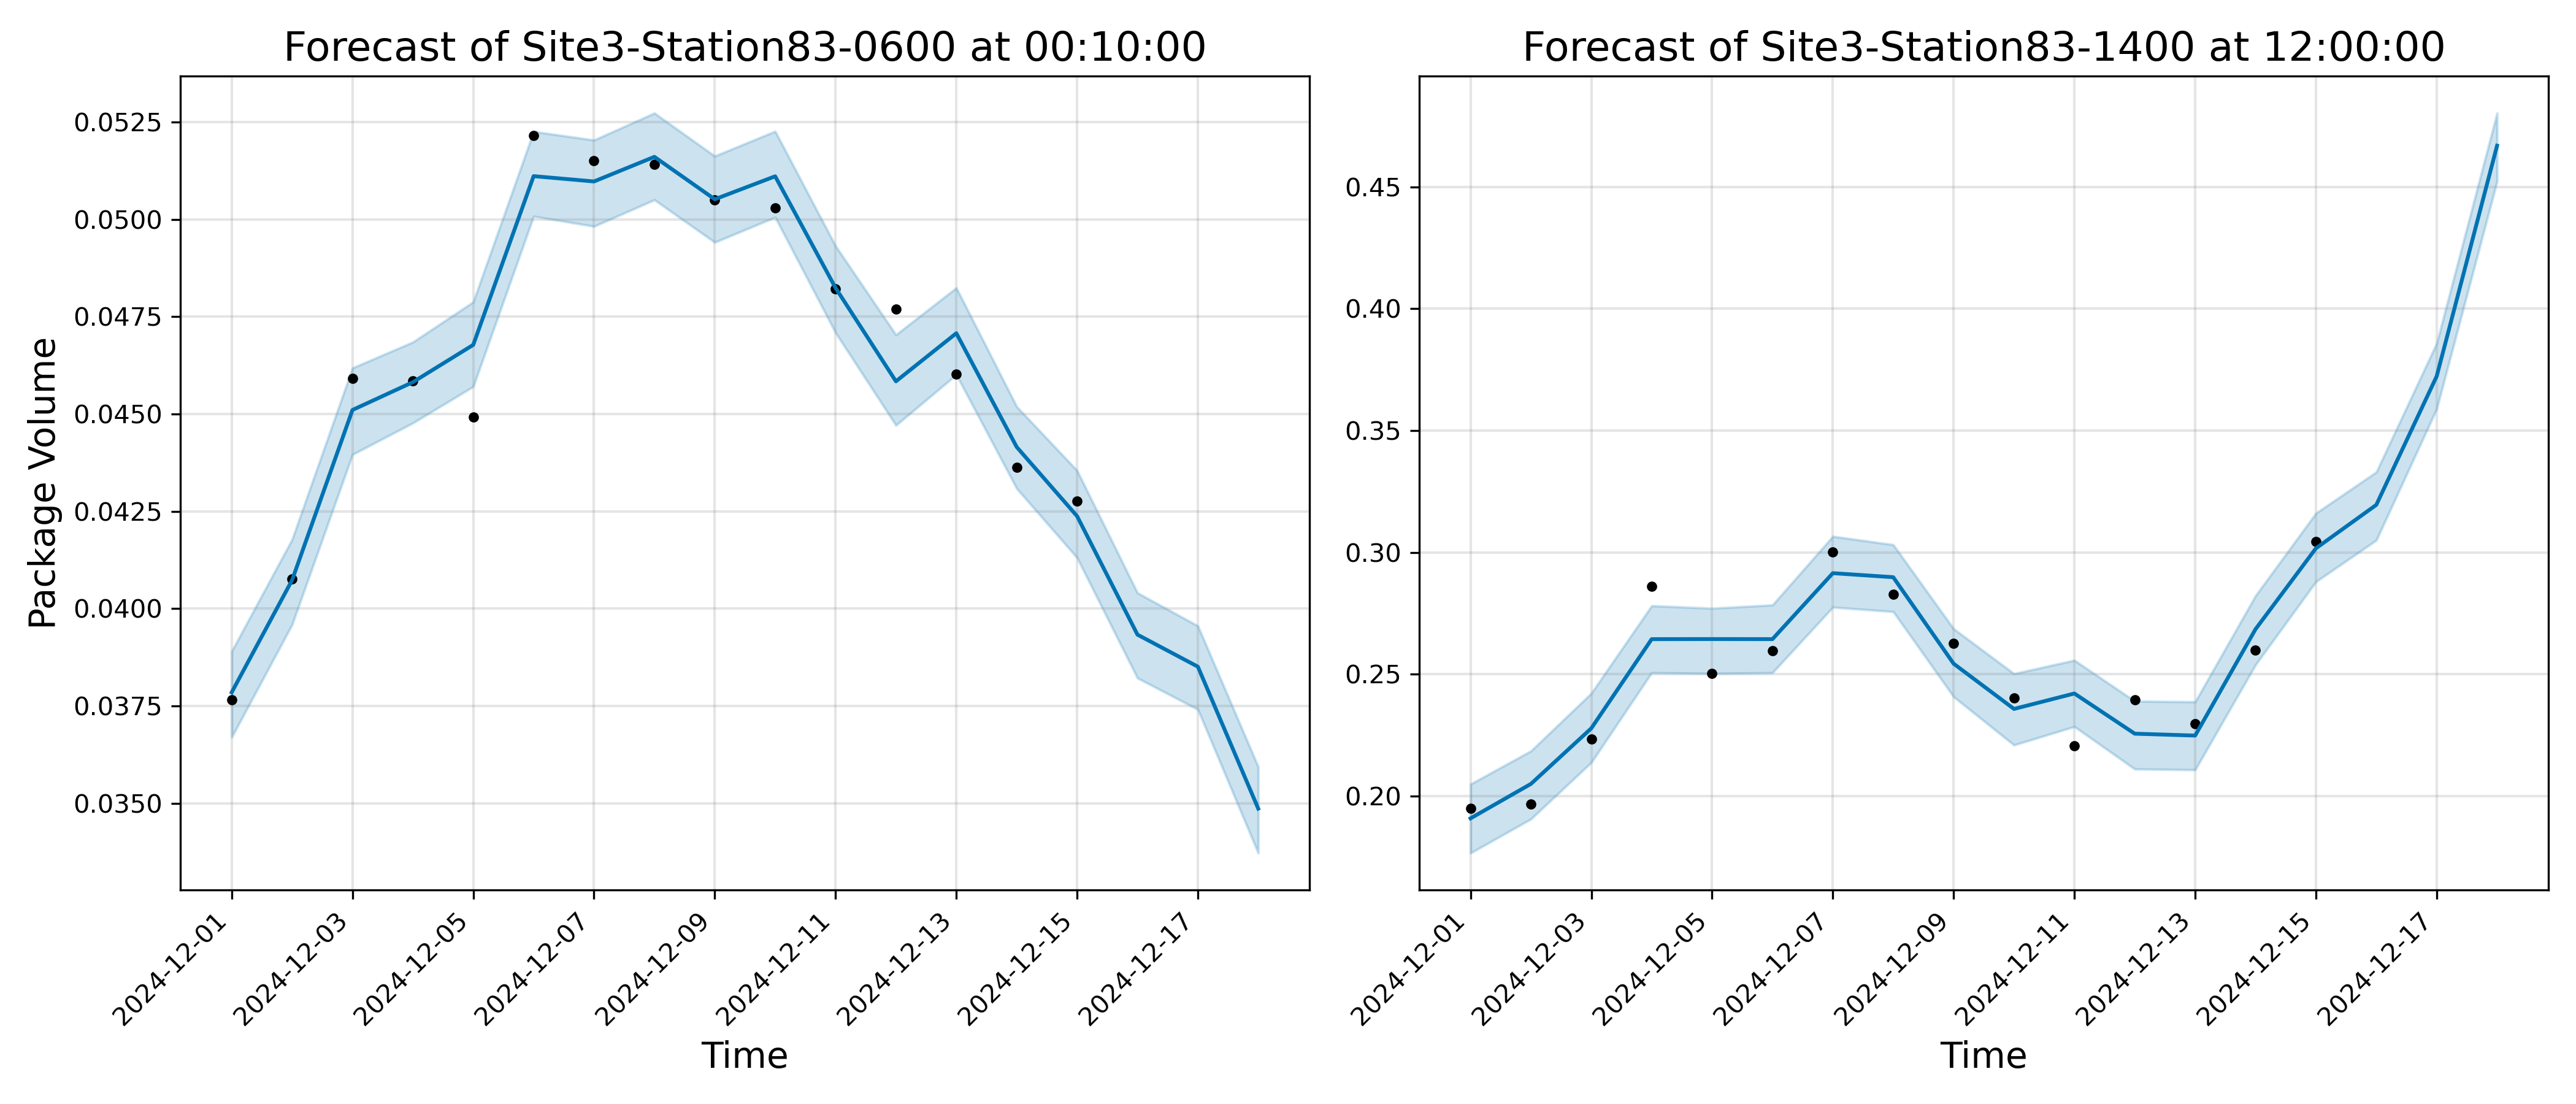
\includegraphics[width=\linewidth]{forecast_comparison.png}
	\caption{场地 3 - 站点 83 特定时段预测折线图}
	\label{fig:9}
\end{figure}

可以发现模型准确的捕捉到了两时段包裹比例剧烈波动的趋势,置信区间在很窄的范围内,这进一步说明我们的模型是有效的。

“场地 3 - 站点 83 – 0600”和“场地 3 - 站点 83 – 1400”的预测结果如表\ref{tab:6}所示。

\begin{table}[htbp]
\centering
\caption{包裹量预测数据汇总(场地3 - 站点83)}
\label{tab:parcel_forecast}
\footnotesize
\begin{tabular}{@{}llcccccc@{}}
\toprule
\textbf{线路编码} & \textbf{小时} & \textbf{:00} & \textbf{:10} & \textbf{:20} & \textbf{:30} & \textbf{:40} & \textbf{:50} \\
\midrule
\multirow{9}{*}{\shortstack{场地3 - 站点83 \\ - 0600}}
& 21 & 77 & 123 & 49 & 70 & 95 & 49 \\
& 22 & 52 & 237 & 193 & 93 & 69 & 38 \\
& 23 & 136 & 77 & 107 & 186 & 137 & 81 \\
& 00 & 216 & 197 & 231 & 73 & 143 & 116 \\
& 01 & 254 & 139 & 139 & 80 & 65 & 234 \\
& 02 & 202 & 172 & 68 & 107 & 54 & 172 \\
& 03 & 133 & 63 & 148 & 240 & 144 & 147 \\
& 04 & 62 & 60 & 165 & 234 & 110 & 99 \\
& 05 & 155 & 255 & 83 & 77 & 331 & 193 \\
\midrule
\multirow{3}{*}{\shortstack{场地3 - 站点83 \\ - 1400}}
& 11 & 55 & 126 & 201 & 433 & 192 & 10 \\
& 12 & 175 & 559 & 131 & 172 & 245 & 98 \\
& 13 & 3 & 16 & 16 & 10 & 59 & 31 \\
\bottomrule
\end{tabular}
\end{table}















\section{问题二模型的建立与求解}
\subsection{问题二概述}
短途运输调度问题要求在既定的发运节点限制下,依据已预测的货量数据,生成每条线路的运输需求,并合理分配车辆资源,完成车辆调度。调度结果需同时优化以下多个目标:
构造调度优化问题,目标为:

	•	最大化自有车辆周转率
 
	•	最大化车辆均包裹率
 
	•	最小化总成本

满足以下约束:

	•	每条线路的发运时间不晚于发运节点

    •	每一车队可用车辆数有限
 
	•	每辆自有车的调度需满足可再发条件
 
	•	串点任务不能超过3条线路
 
	•	外部车辆数量无限
 
\subsection{问题二分析}
\subsubsectionautorefname问题二聚焦于在考虑车辆可复用性约束的前提下,如何对各线路在各时间片内的货运需求进行合理调度,以最小化整体运输成本。在问题一中,车辆在各线路之间不可复用,调度方案相对静态;而在问题二中,引入了“车辆可在串联线路之间复用”的动态调度机制,显著增加了解的复杂性与实际可行性。

本问题要求在满足各项基本约束(如货物必须在当日完成运输、每辆车每日可调度一次、车辆使用优先级等)的前提下,对所有货物运输需求进行合理分配,选择自有车辆或外部承运方式,以实现成本最优化。
\subsection{模型建立与求解}
\subsubsection{启发式算法}

为解决问题二中提出的运输需求确定与车辆调度任务,我们设计了一种启发式贪心算法,用于在满足全部约束条件的前提下,构造可行解并实现初步优化。该算法以时间片为基本单位(10分钟),逐步累加各条运输线路在当前时间片内的新增货量;当累计货量达到车辆满载阈值(1000个包裹)时,即生成一个运输需求。

为了确保所有运输需求在规定的发运节点前被执行完毕,我们在每一时间片内即时进行车辆调度。调度策略遵循以下优先级顺序:

1.	自有车辆优先调度:若对应线路当前存在空闲自有车辆,则直接分配以完成当前需求;

2.	串联线路车队支援:若本线路无空闲车辆,则尝试从与该线路存在“串点关系”的其他线路中调度车队所辖车辆;

3.	外部承运保证完成:若上述两种资源均不可用,则调用外部承运商以完成该需求。

求解结果:

\subsubsection{类 VRPTW 框架的引入与改进}
\section{问题三模型建立与求解}
\subsection{问题分析}
\subsubsection{问题概述}
在问题二的基础上,问题三引入了一种标准容器的可选使用方案。该容器在短途运输中可有效缩短操作时间(装卸时间由原来的45分钟缩短至10分钟),进而提升车辆周转效率;但其缺点在于装载能力下降,每辆车可装载的包裹量由1000个降至800个。

本问题要求在运输时效约束下,重新确定运输需求、车辆分配及是否使用标准容器的策略,并以自有车辆周转率最大化、车辆均包裹量最大化、总运输成本最小化为优化目标,输出新的调度方案。
\subsubsection{变量变化与模型影响}
标准容器的引入,导致原调度模型中若干关键参数发生变化:
这种变化构成了典型的权衡问题:装载能力下降可能会导致运输需求总数上升(增加车辆次数与成本),但装卸时间的缩短则显著提升周转空间与调度灵活性,可能减少对外部车辆的依赖,从而降低整体运输成本。

\subsection{模型的建立与求解}
\subsubsection{启发式算法}
针对问题三,我们同样设计了一种启发式调度算法,以有效整合标准容器的使用策略与车辆资源的优化配置。在该算法中,我们引入子集合(subset)划分机制,将具备串点条件的线路划分为若干互不相同,但可能包含相同线路的子集合,每个子集合对应一组可共同发运的线路集合。

在调度过程中,算法以固定时间片(10分钟)为单位,逐步对每个子集合的包裹量进行动态累积。在每一时间片中,分别统计达到两种发运阈值(标准容器阈值800件与常规装载阈值1000件)的子集合,并依据可用资源情况将其划分为两类:一类为可由自有车辆承运的子集合,另一类为需依赖外部承运商的子集合。

进一步地,考虑到成本最小化目标,在每一类中,我们按各子集合所对应的最大线路运输成本从低到高进行排序,并优先调度成本最低的子集合,以实现整体运输支出的优化控制。

在发运方式的判定方面,若子集合的累计包裹量属于[800, 1000],则优先采用标准容器进行发运,以提升装卸效率;而当货量超过1000件时,则采用常规方式发运,以充分利用车辆运载能力。

该算法策略在保证发运及时性的前提下,综合考虑了车辆资源利用、成本结构优化与标准容器的适用性,能够在动态约束条件下生成具有较高实用性的调度方案。
	\begin{enumerate}
		\item 假设1;
		\item 假设2;
		\item 假设3;
		\item 假设4;
		\item 假设5
	\end{enumerate}
	\section{符号说明}
	\begin{center}
		\begin{tabularx}{0.7\textwidth}{c@{\hspace{1pc}}|@{\hspace{2pc}}X}
			\Xhline{0.08em}
			符号 & \multicolumn{1}{c}{符号说明}\\
			\Xhline{0.05em}
			$\delta$ & 符号1\\
			$\beta$ & 符号2\\
			$\alpha$ & 符号3\\
			$r$ & 符号4\\
			$\gamma$ & 符号5\\
			$l$ & 符号6\\
			$l_{y}$ & 符号7\\
			$\vec{x}_{1},\vec{y}_{1},\vec{z}_{1}$ & 符号8\\
			$\vec{\hat{x}}_{1},\vec{\hat{y}}_{1},\vec{\hat{z}}_{1}$ & 符号9\\
			$\theta$ & 符号10\\
			$l_{y}(i)$ & 编号为 $i$ 符号11\\
			$\theta_{i}$ & 编号为 $i$ 符号12\\
			\Xhline{0.08em}
		\end{tabularx}
	\end{center}

	\section{模型的建立与求解}
模型的建立与求解模型的建立与求解模型的建立与求解模型的建立与求解模型的建立与求解模型的建立与求解模型的的建立与求解模型的建立与求解模型的建立与求解模型的建立与求解模型的建立与求解模型的建立与求解模型的建立与求解模型的建立与求解模型的建立与求解模型的建立与求解模型的建立与求解模型的建立与求解模型的建立与求解。

模型的建立与求解模型的建立与求解模型的建立与求解模型的建立与求解模型的建立与求解模型的建立与求解模型的建立与求解模型的建立与求解模型的建立与求解模型的建立与求解模型的建立与求解模型的建立与求解模型的建立与求解模型的建立与求解模型的建立与求解。
	\subsection{模型的准备}
模型的准备模型的准备模型的准备模型的准备模型的准备模型的准备模型的准备模型的准备模型的准备模型的准备模型的准备模型的准备。模型的准备模型的准备模型的准备模型的准备模型的准备模型的准备模型的准备模型的准备模型的准备模型的准备模型的准备模型的准备模型的准备。

模型的准备模型的准备模型的准备模型的准备模型的准备模型的准备模型的准备模型的准备模型的准备模型的准备模型的准备模型的准备模型的准备。

	\subsection{模型一的建立}
 模型一的建立模型一的建立模型一的建立模型一的建立模型一的建立模型一的建立模型一的建立模型一的建立模型一的建立模型一的建立模型一的建立模型一的建立模型一的建立模型一的建立模型一的建立模型一的建立模型一的建立模型一的建立模型一的建立模型一的建立模型一的建立模型一的建立模型一的建立模型一的建立模型一的建立。
	效果见\cref{fig:1}。
	\begin{figure}[h]
		\centering
		\includegraphics[width=0.4\textwidth]{figure/image.png}
		\caption{content}\label{fig:1}
	\end{figure}
 模型一的建立模型一的建立模型一的建立模型一的建立模型一的建立模型一的建立模型一的建立模型一的建立模型一的建立模型一的建立模型一的建立模型一的建立模型一的建立模型一的建立模型一的建立模型一的建立模型一的建立。

 模型一的建立模型一的建立模型一的建立模型一的建立模型一的建立模型一的建立模型一的建立模型一的建立模型一的建立模型一的建立模型一的建立模型一的建立。模型一的建立。
	\subsection{模型二的建立}
 
	结果见\cref{tab:1}。
 
	\begin{table}[h]
		\centering
		\caption{content}\label{tab:1}
		\begin{tabularx}{0.7\textwidth}{c@{\hspace{1pc}}|@{\hspace{2pc}}X}
		\Xhline{0.08em}
		符号 & \multicolumn{1}{c}{符号说明}\\
		\Xhline{0.05em}
		$\delta$ & 赤纬角\\
		$\beta$ & 经度\\
		$\alpha$ & 纬度\\
		$r$ & 地球半径\\
		$\gamma$ & 太阳光与杆所成的夹角\\
		$l$ & 杆的长度\\
		$l_{y}$ & 杆的影子长度\\
		$\vec{x}_{1},\vec{y}_{1},\vec{z}_{1}$ & 由杆的位置所生成的切平面的正交基\\
		$\vec{\hat{x}}_{1},\vec{\hat{y}}_{1},\vec{\hat{z}}_{1}$ & 由杆的位置所生成的切平面的单位正交基\\
		$\theta$ & 影子与北方的夹角\\
		$l_{y}(i)$ & 编号为 $i$ 的数据对应的影子长度\\
		$\theta_{i}$ & 编号为 $i$ 的数据对应的影子角度\\			\Xhline{0.08em}
		\end{tabularx}
	\end{table}
 
	\subsection{模型三的建立}
	模型三的建立模型三的建立模型三的建立模型三的建立模型三的建立模型三的建立模型三的建立模型三的建立模型三的建立模型三的建立模型三的建立模型三的建立模型三的建立模型三的建立模型三的建立模型三的建立模型三的建立模型三的建立模型三的建立模型三的建立模型三的建立模型三的建立。

	\section{模型的检验}
	模型的检验模型的检验模型的检验模型的检验模型的检验模型的检验模型的检验模型的检验模型的检验模型的检验模型的检验模型的检验模型的检验模型的检验模型的检验模型的检验模型的检验模型的检验模型的检验模型的检验模型的检验模型的检验模型的检验。

	\section{模型的评价与改进}
	模型的评价与改进模型的评价与改进模型的评价与改进模型的评价与改进模型的评价与改进模型的评价与改进模型的评价与改进模型的评价与改进模型的评价与改进模型的评价与改进模型的评价与改进模型的评价与改进模型的评价与改进模型的评价与改进模型的评价与改进模型的评价与改进模型的评价与改进模型的评价与改进。
 
	\subsection{模型的优点}
	模型的优点。模型的优点模型的优点模型的优点模型的优点模型的优点模型的优点模型的优点模型的优点模型的优点模型的优点模型的优点模型的优点模型的优点模型的优点模型的优点。
	\subsection{模型的缺点}
	模型的缺点。模型的缺点模型的缺点模型的缺点模型的缺点模型的缺点模型的缺点模型的缺点模型的缺点模型的缺点模型的缺点模型的缺点模型的缺点模型的缺点模型的缺点模型的缺点模型的缺点模型的缺点模型的缺点模型的缺点。
	\subsection{模型的改进}
	模型的改进。模型的改进模型的改进模型的改进模型的改进模型的改进模型的改进模型的改进模型的改进模型的改进模型的改进模型的改进模型的改进模型的改进模型的改进模型的改进模型的改进模型的改进模型的改进模型的改进模型的改进模型的改进模型的改进模型的改进模型的改进模型的改进模型的改进模型的改进。

	\phantomsection
	\addcontentsline{toc}{section}{参考文献}
	\bibliography{ref}

	\newpage
	\appendix
	\ctexset{section={
		format={\zihao{-4}\heiti\raggedright}
	}}
	\begin{center}
		\heiti\zihao{4} 附\hspace{1pc}录
	\end{center}
	\section{问题一的 MATLAB 代码}
	
 \begin{matlab}
    clc,clear
    %第七题
    R71 = 1;
    R72 = 2;
    T7 = 1;
    K7 = 1;
    N7=10^5;
    G71=tf(R72,R71);
    G72=tf(1,[T7 1]);
    G73=tf(1,[T7 0]);
    G74=tf([N7*T7 0],[T7 N7]);
    G75=tf([N7*K7*T7 N7*K7],[T7 N7]);
    G76=tf([K7*T7 K7],[T7 0]);
    
    subplot(2,3,1)
    step(G71)
    xlabel('$t$','interpreter','latex', 'FontSize', 12);
    ylabel('$y$','interpreter','latex', 'FontSize', 12);
    title('比例环节');
	
 \end{matlab}
 \section{问题一的 python 代码}
  \begin{python}
      import torch
      import numpy as np
      import pandas as pd
      for i in range(100):
          print('demo')
  \end{python}
\end{document}